\documentclass[11pt,a4paper]{report}
\usepackage[utf8]{inputenc}
\usepackage{a4wide}
\usepackage[english]{babel}
\usepackage{graphicx}
\usepackage{siunitx}
\usepackage[margin=1in]{geometry}
\usepackage{lastpage}		
\newcommand{\npar}{\vspace{0.5cm} \par \noindent} 
\usepackage[utf8]{inputenc}
\usepackage{newunicodechar}
\usepackage{float}
\usepackage{graphicx}
\usepackage{array}
%\usepackage{subcaption}
\usepackage{hyperref}
\usepackage{amsmath}
\usepackage{cleveref}
\usepackage{amsmath}
\usepackage{circuitikz}
\usepackage{textcomp}
\usepackage{multicol}
\usepackage{gensymb}
\usepackage{rotating}
\usepackage{subcaption}
\usepackage{fixltx2e}
\usepackage{notoccite}

\usepackage[final]{pdfpages}
\usepackage{enumerate}
\usepackage{chemformula}
\usepackage{listings}
%\usepackage{subfig}
\usepackage{xcolor}
\usepackage{pdfpages}
\usepackage{nomencl}
\makenomenclature

\usepackage{etoolbox}
\renewcommand\nomgroup[1]{%
  \item[\bfseries
  \ifstrequal{#1}{A}{Abbreviations}{%
  \ifstrequal{#1}{L}{Letters}{%
  \ifstrequal{#1}{G}{Greek Symbols}{}}}%
]}

\usepackage{booktabs}
\usepackage{longtable}
\usepackage{array}
\usepackage{ragged2e}
\usepackage{pdflscape}
\usepackage{eurosym}
\usepackage{amssymb}


%%%%%%%%%%%%%%%%%%%%%%%%%% For python code
% Default fixed font does not support bold face
\DeclareFixedFont{\ttb}{T1}{txtt}{bx}{n}{10} % for bold
\DeclareFixedFont{\ttm}{T1}{txtt}{m}{n}{10}  % for normal

% Custom colors
\usepackage{color}
\definecolor{deepblue}{rgb}{0,0,0.5}
\definecolor{deepred}{rgb}{0.6,0,0}
\definecolor{deepgreen}{rgb}{0,0.5,0}

\usepackage{listings}

% Python style for highlighting
\newcommand\pythonstyle{\lstset{
language=Python,
basicstyle=\ttm,
otherkeywords={self},             % Add keywords here
keywordstyle=\ttb\color{deepblue},
emph={MyClass,__init__},          % Custom highlighting
emphstyle=\ttb\color{deepred},    % Custom highlighting style
stringstyle=\color{deepgreen},
frame=tb,                         % Any extra options here
showstringspaces=false,
breaklines = true,
}}


% Python environment
\lstnewenvironment{python}[1][]
{
\pythonstyle
\lstset{#1}
}
{}

% Python for external files
\newcommand\pythonexternal[2][]{{
\pythonstyle
\lstinputlisting[#1]{#2}}}
%%%%%%%%%%%%%%%%%%%%%%%%%%%%%%%

\begin{document}


\includepdf[pages=-]{TitlePage.pdf}
\newpage
\vspace*{\fill}
\noindent
''The author gives permission to make this master dissertation available for consultation and to copy parts of this master dissertation for personal use. In all cases of other use, the copyright terms have to be respected, in particular with regard to the obligation to state explicitly the source when quoting results from this master dissertation.''

\addvspace{2cm}

\noindent Ghent, June [year]\\
\noindent [Name]

\newpage
\addcontentsline{toc}{chapter}{Preface}
\section*{Preface}
\npar
\noindent
[Preface]

%  Overzichtsbladzijde met samenvatting

\newpage
\addcontentsline{toc}{chapter}{Abstract}
{
\setlength{\baselineskip}{12pt}
\setlength{\parindent}{0pt}
\setlength{\parskip}{6pt}



\renewcommand{\baselinestretch}{1.1}
\noindent \fontseries{bx}
\fontsize{14pt}{21pt}
\selectfont
\vspace{-2.5cm}
\begin{center}
Title\\
\renewcommand{\baselinestretch}{1.3}
\fontseries{m}
\fontsize{12pt}{14pt}
\selectfont
\vspace{0.5cm}
[Name]\\
\end{center}

\renewcommand{\baselinestretch}{1.3}
\fontseries{m}
\fontsize{12pt}{12pt}
\selectfont

Supervisor: \\
Counsellors: \\

Master's dissertation submitted in order to obtain the academic degree of\\
\textsc{Master of Science in Electromechanical Engineering}\\

Departement of Electromechanical, Systems and Metal Engineering\\
Chair: \\
Faculty of Engineering and Architecture\\
Ghent University\\
Academic year 2025--2026\\

\textbf{Summary}



\textbf{Keywords:} 
}

\newpage % strikt noodzakelijk om een header op deze blz. te vermijden
\addcontentsline{toc}{chapter}{Extended Abstract}
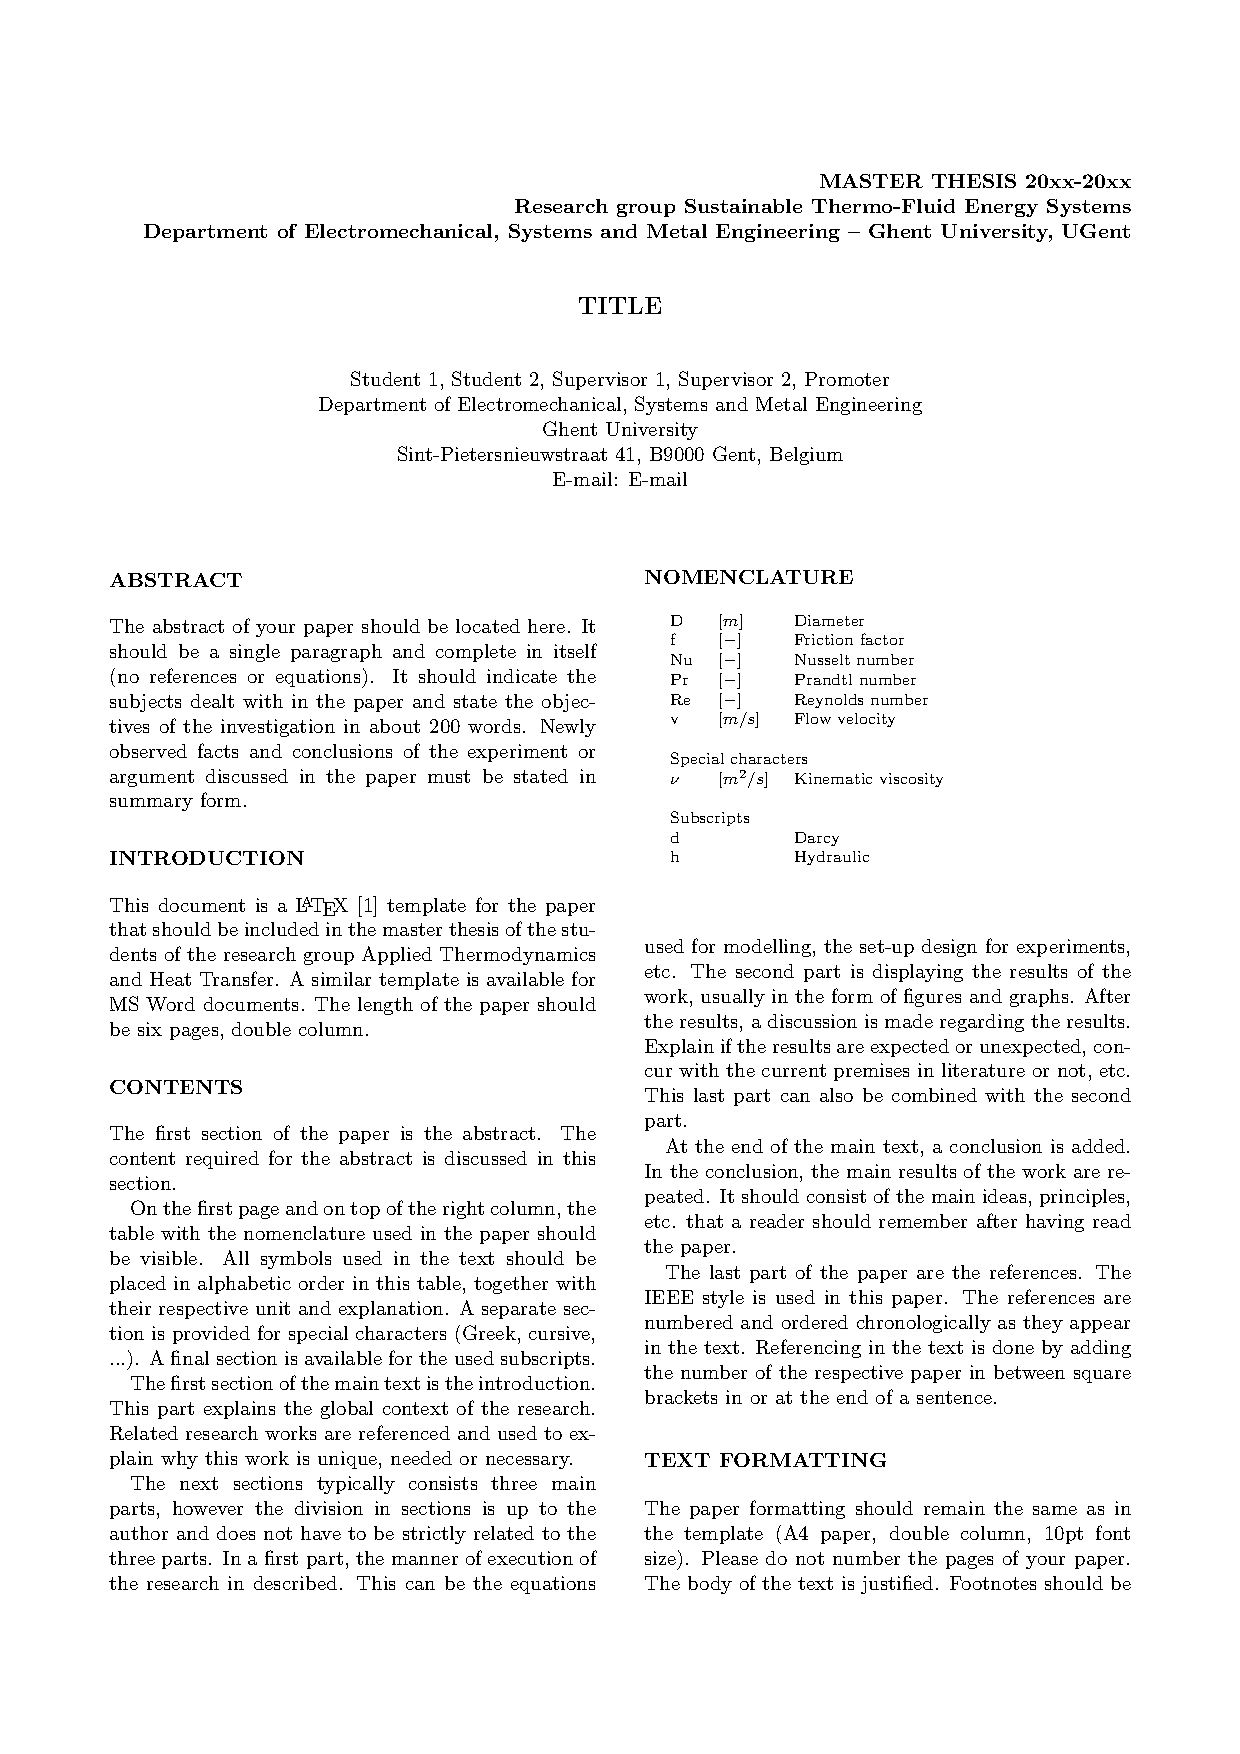
\includepdf[pages=-]{template_6_page_paper_Latex.pdf}
\addcontentsline{toc}{chapter}{Table of Contents}
\tableofcontents
\newpage
\addcontentsline{toc}{chapter}{List of Figures}
\listoffigures

\newpage
\addcontentsline{toc}{chapter}{List of Tables}
\listoftables

\newpage
\addcontentsline{toc}{chapter}{Nomenclature}
\nomenclature[A]{\textbf{DER}}{\textbf{Distributed Energy Resource}}
\nomenclature[A]{\textbf{ANF}}{\textbf{Annuity Factor}}
\nomenclature[A]{\textbf{BESS}}{\textbf{Battery Energy Storage System}}
\nomenclature[A]{\textbf{COP}}{\textbf{Coefficient of Performance} (HP efficiency metric)}
\nomenclature[A]{\textbf{DHW}}{\textbf{Domestic Hot Water}}
\nomenclature[A]{\textbf{HPS}}{\textbf{Heat Pump System}}
\nomenclature[A]{\textbf{HP}}{\textbf{Heat Pump}}
\nomenclature[A]{\textbf{MILP}}{\textbf{Mixed-Integer Linear Programming}}
\nomenclature[A]{\textbf{MINLP}}{\textbf{Mixed-Integer Non-Linear Programming}}
\nomenclature[A]{\textbf{OP}}{\textbf{Operation Point} (for linearization reference)}
\nomenclature[A]{\textbf{PV}}{\textbf{Photovoltaic}}
\nomenclature[A]{\textbf{PWL}}{\textbf{Piecewise Linear} (approximation)}
\nomenclature[A]{\textbf{SH}}{\textbf{Space Heating}}
\nomenclature[A]{\textbf{TES}}{\textbf{Thermal Energy Storage}}
\nomenclature[A]{\textbf{TRY}}{\textbf{Test Reference Year} (used for clustered data)}


\nomenclature[L]{$\boldsymbol{A_{\text{ref.}}}$}{Surface area of one PV module (reference)}
\nomenclature[L]{$\boldsymbol{c_{w}}$}{Specific heat capacity of water [J/(kg K)]}
\nomenclature[L]{$\boldsymbol{C}$}{Electricity Cost [\euro]}
\nomenclature[L]{$\boldsymbol{CC}$}{Cooling Capacity during defrost operation [W]}
\nomenclature[L]{$\boldsymbol{D}$}{Comfort Index (Quantifies thermal discomfort) [\degree C]}
\nomenclature[L]{$\boldsymbol{d}$}{TES diameter}
\nomenclature[L]{$\boldsymbol{DT}$}{Acceptable Water Temperature Differential [\degree C]}
\nomenclature[L]{$\boldsymbol{FD}$}{Fluid Density [g/L]}
\nomenclature[L]{$\boldsymbol{f}$}{Objective function (Total minimized cost/discomfort)}
\nomenclature[L]{$\boldsymbol{G_{\text{POA}}}$}{Solar irradiance in the Plane of Array [W/m$^2$]}
\nomenclature[L]{$\boldsymbol{h}$}{Height of TES}
\nomenclature[L]{$\boldsymbol{MDD}$}{Max Defrost Duration [s]}
\nomenclature[L]{$\boldsymbol{P_{el,HP}}$}{Electric power consumed by HP [W]}
\nomenclature[L]{$\boldsymbol{P_{0}}$}{Rated heating power of EWH [W]}
\nomenclature[L]{$\boldsymbol{P_{\text{DC}}}$}{DC power output of PV system [W]}
\nomenclature[L]{$\boldsymbol{P_{\text{STC}}}$}{Nominal DC power for one PV module [W]}
\nomenclature[L]{$\boldsymbol{\dot{Q}_{HP}}$}{Heat output of HP [W]}
\nomenclature[L]{$\boldsymbol{Q_{\text{N}}}$}{Nominal capacity of TES}
\nomenclature[L]{$\boldsymbol{Q_{t}}$}{Stored energy in TES at time $t$}
\nomenclature[L]{$\boldsymbol{R}$}{Water heater thermal resistance [K$\cdot$day/kWh]}
\nomenclature[L]{$\boldsymbol{SH}$}{Specific Heat of fluid [J/(g$\cdot$\degree C)]}
\nomenclature[L]{$\boldsymbol{T_{\text{amb}}}$}{Ambient outdoor air temperature (OAT) [\degree C]}
\nomenclature[L]{$\boldsymbol{T_{\text{biv}}}$}{Bivalence temperature (Reference design point) [K]}
\nomenclature[L]{$\boldsymbol{T_{\text{cell}}}$}{PV cell temperature [\degree C]}
\nomenclature[L]{$\boldsymbol{T_{cw}}$}{Temperature of cold mixing water [\degree C]}
\nomenclature[L]{$\boldsymbol{T_{\text{exp}}}$}{Most desirable tap water temperature [\degree C]}
\nomenclature[L]{$\boldsymbol{T_{\text{High,mean}}}$}{Mean temp.\ of delivered hot water [K]}
\nomenclature[L]{$\boldsymbol{T_{in}}$}{Water temperature in EWH/TES tank [\degree C]}
\nomenclature[L]{$\boldsymbol{T_{\text{inlet}}}$}{Temperature of cold water flowing into the tank [\degree C]}
\nomenclature[L]{$\boldsymbol{T_{max}}$}{Maximum temperature EWH tank can withstand [\degree C]}
\nomenclature[L]{$\boldsymbol{T_{ref}}$}{Reference temperature [\degree C]}
\nomenclature[L]{$\boldsymbol{T_{tap}}$}{Current tap water temperature [\degree C]}
\nomenclature[L]{$\boldsymbol{u(t)}$}{On/off status variable of EWH (binary) [-]}
\nomenclature[L]{$\boldsymbol{v_{\text{wind}}}$}{Wind velocity [m/s]}
\nomenclature[L]{$\boldsymbol{x(t)}$}{Switch-on signal of EWH (binary) [-]}
\nomenclature[L]{$\boldsymbol{y(t)}$}{Switch-off signal of EWH (binary) [-]}
\nomenclature[L]{$\boldsymbol{y_{HP,TES}}$}{Binary on/off status of HP for a given TES [-]}


\nomenclature[G]{$\boldsymbol{\alpha}$}{User preference factor (Weighting factor for cost) [-]}
\nomenclature[G]{$\boldsymbol{\beta}$}{Weighting factor for comfort $(\alpha+\beta=1)$ (EWH) [-]}
\nomenclature[G]{$\boldsymbol{\gamma}$}{Coefficient for TES lateral surface loss}
\nomenclature[G]{$\boldsymbol{\gamma_{\text{pdc}}}$}{Temperature coefficient of power (PV) [\%/\degree C]}
\nomenclature[G]{$\boldsymbol{\delta(t)}$}{Auxiliary variable for PWL approximation (binary) [-]}
\nomenclature[G]{$\boldsymbol{\Delta t}$}{Time step size for heat generation [s]}
\nomenclature[G]{$\boldsymbol{\Delta \tau}$}{Longer discretization period for TES/Supply [s]}
\nomenclature[G]{$\boldsymbol{\eta}$}{Efficiency (General) [-]}
\nomenclature[G]{$\boldsymbol{\eta_{\text{HP}}}$}{HP efficiency factor [-]}
\nomenclature[G]{$\boldsymbol{\kappa}$}{Electricity price [\euro/kWh]}
\nomenclature[G]{$\boldsymbol{\lambda}$}{Thermal conductivity of water [W/(m K)]}
\nomenclature[G]{$\boldsymbol{\mu}$}{Scale factor (EWH objective function) [\degree C/\euro]}
\nomenclature[G]{$\boldsymbol{\rho_{w}}$}{Water density [kg/m$^3$]}
\nomenclature[G]{$\boldsymbol{\theta}$}{Time step ratio $(\Delta \tau / \Delta t)$ [-]}

\printnomenclature
\chapter{Introduction}
\label{intro}




\section{The imperative for decarbonization in the building sector}
The global energy transition is increasingly focused on the urgent need to reduce greenhouse gas emissions and mitigate climate change.
A critical battleground in this transition is the building sector, which remains a significant contributor to energy use and carbon emissions.
For instance, in Belgium alone, the building sector\footnote{In this context, the building sector definition follows the European climate reporting categories, which encompass direct emissions from fossil fuel combustion in residential and tertiary (commercial/institutional) buildings, as well as energy-related emissions from the agriculture and fishery sectors.} is responsible for approximately 20\% of total carbon dioxide ($CO_2$) emissions in 2022 \cite{EU_Climate_Action_Belgium_2023}.
To meet ambitious climate goals, such as those outlined by the European Union, there is a pressing need to decarbonize the heat supply for buildings.
Under the \textit{European Climate Law}, the EU is legally committed to a progressive decarbonization pathway: a net greenhouse gas (GHG) emissions reduction of at least 55\% by 2030 (compared to 1990 levels), an intermediate target of 90\% by 2040, and the ultimate goal of climate neutrality by 2050 \cite{EU_Climate_Law_2021, EU_2040_Target_2026}.
For the building sector specifically, the revised \textit{Energy Performance of Buildings Directive} (EPBD) mandates that all new buildings must be Zero-Emission Buildings (ZEB) by 2030, with a complete phase-out of fossil-fuel-based heating systems required by 2040 \cite{EPBD_2024}.
The significance of the building sector in this context stems largely from the high carbon intensity of thermal energy demands.
Space heating (SH) and domestic hot water heating (DHW) account for approximately 77,6\% of the total energy consumption in residential buildings in Belgium in 2023 \cite{Eurostat_Energy_Consumption_2023}.
Because much of this demand is currently met through the direct combustion of fossil fuels, such as natural gas and heating oil, the thermal energy share is the primary driver of the sector's operational $CO_2$ emissions.
This transition relies heavily on shifting away from fossil-fuel-based systems, such as gas boilers, toward electrification using renewable energy sources (RES) \cite{EnergyVille_PATHS2050_Residential_2025} \cite{Esen2006}.

\section{The role of heat pumps and challenges in refurbishment}
Heat pump systems (HPSs) have emerged as a key technology for electrifying space heating (SH) and domestic hot water (DHW) production\cite{Esen2006}.
Their ability to generate thermal energy efficiently from electricity makes them a cornerstone of sustainable building energy systems.
However, the widespread adoption of heat pumps faces significant economic barriers, particularly in the refurbishment of existing buildings.
In these scenarios, heat pumps often compete with gas boilers, which traditionally have lower investment costs.
Furthermore, older buildings often utilize radiator heating systems requiring high flow temperatures (up to $70^{\circ}C$), unlike modern underfloor heating.
Consequently, heat pumps for elevated temperatures are essential for these applications to ensure comfort without extensive renovations.
To increase market penetration and motivate homeowners to switch to low-carbon solutions, HPSs must become more economically competitive. The Flemish government and the heat pump sector have recently established a 
collaborative framework to address these economic barriers and accelerate 
the deployment of HPSs \cite{VEKA2026}.
To shift the market from a 10\% adoption rate toward a 70\% target for 
renovations, the strategy focuses on three primary economic levers.
First, capital barriers are mitigated through substantial direct subsidies, 
where premiums can reach up to €8,000 per installation.
Furthermore, the provision of interest-free or low-interest renovation 
loans allows for the pre-financing of the high upfront costs, aligning 
the investment with long-term energy savings.
Second, a strategic energy tax shift is being implemented to reduce the 
price of electricity relative to fossil fuels, ensuring that HPSs remain 
the most cost-effective solution for daily operation.
Finally, the industry has committed to a "Heat Pump Charter" to enhance 
installation quality and provide standardized technical guidance, ensuring 
that systems are optimized for the specific flow requirements of 
refurbished buildings \cite{VEKA2026}.

\section{The Transition to Renewable Heat Supply: Challenges and Solutions}

The urgent need to reduce dependence on fossil fuels has accelerated the integration of Renewable Energy Sources (RES), such as Photovoltaic (PV) systems, into the built environment.
This shift is a cornerstone of sustainable development, yet the transition toward a fully renewable heat supply introduces a fundamental challenge: the intermittency of sources like solar and wind.
Unlike fossil fuels, where energy supply is constant and dispatchable, the generation of RES fluctuates based on weather conditions.
This stochastic nature poses a direct risk to grid stability and the security of energy supply.

\subsection{Flexibility through Electrification and Storage}
To mitigate these fluctuations and ensure reliability, the electrification of heat demand must be supported by intelligent control and storage technologies.
The following components are essential to framing this transition:

\begin{itemize}
    \item \textbf{Demand Side Management (DSM):} 
        This strategy steers electrical loads to match the availability of renewable generation, optimizing the timing of consumption.
            \item \textbf{Thermal Energy Storage (TES):} 
                By coupling TES units with heat pumps, heat generation can be decoupled from immediate demand. 
                    This provides the necessary flexibility to shift electrical loads to periods when renewable electricity is abundant or cheaper.
                        \item \textbf{Electrical Storage (Batteries):} 
                            Integrating battery systems alongside PV generation further stabilizes the grid by maximizing self-consumption and reducing peak loads on the distribution network.
                            \end{itemize}
                            
                            
                            
                            While the synergy between PV systems, heat pumps, and storage technologies offers a robust path toward a fossil-free future, it introduces significant layers of control complexity.
                            The primary challenge lies in balancing the maximization of energy savings and grid support with the non-negotiable requirement of maintaining user comfort, such as consistent domestic hot water temperatures and a stable indoor climate.
                            
                            
                    



\section{The design gap: From static rules to dynamic optimization}
Despite the clear benefits of hybrid energy systems, current design practices remain a bottleneck.
European normative standards for dimensioning HPSs (such as EN 15450 \cite{EN15450_2007}) typically rely on static rules and single operating points.
These procedures often determine the size of individual components sequentially, neglecting the complex interdependencies between the heat pump, storage sizing, and control strategies.
This static approach can lead to sub-optimal designs.
Furthermore, the optimal size of a system is heavily dependent on its operation; a system designed without considering its control strategy may be oversized and economically inefficient \cite{Dongellini2017}.
Therefore, to achieve a truly optimal and sustainable design, dimensioning and operation must be optimized simultaneously.  By optimizing
the system, we can reduce investment costs significantly about 45\% in comparison to normative standards,
while maintaining security of supply and not increasing electrical energy consumption\cite{Krutzfeldt2021}.



\section{Thesis Objective}
This thesis aims to bridge this gap by developing a comprehensive design tool in Python using MILP.
The tool will determine the optimal economic sizing of a hybrid energy system comprising a High-Temperature Heat Pump (HTHP), Photovoltaics (PV), Battery storage, and Thermal Energy Storage (TES).
By incorporating detailed modeling of system dynamics and component interdependencies, this work seeks to provide a solution that is not only economically viable but also environmentally sustainable, accelerating the decarbonization of the residential heating sector.

\subsection{Case Study Application: Transitioning M-accent from Gas to Hybrid Electrification}

The practical necessity for advanced optimization is exemplified by the M-accent case study, which currently relies on two 80~kW gas boilers for its primary heat supply. Decarbonizing such a system requires a transition to a hybrid energy architecture. To replace the existing 160~kW fossil-fuel capacity, this thesis proposes a system integrating a High-Temperature Heat Pump (HTHP), Photovoltaics (PV), Battery Energy Storage Systems (BESS), and Thermal Energy Storage (TES).

The integration of these technologies presents a complex sizing problem that exceeds the capabilities of static design standards like EN 15450 \cite{EN15450_2007}. Specifically, the design tool developed in this work addresses the following technical challenges identified in literature:

\begin{itemize}
    \item \textbf{HTHP Performance:} Unlike traditional boilers, the capacity and Coefficient of Performance (COP) of HTHPs are highly dependent on source and sink temperatures. Following the methodology of Krützfeldt et al. \cite{Krutzfeldt2021}, the tool utilizes MILP to account for these non-linearities through piecewise linear approximations or regressive modeling based on manufacturer data, such as the Daikin EWYE-CZ.
    
    \item \textbf{Storage Synergies:} The tool optimizes the trade-off between electrochemical (Battery) and thermal (TES) storage. While batteries facilitate PV self-consumption, TES allows for the decoupling of heat production from demand, which is crucial for managing the peak loads previously handled by the 80~kW boilers \cite{Steen2015, Krien2020oemofsolph}.
    
    \item \textbf{Economic Dispatch:} By utilizing MILP, the tool simultaneously determines the optimal investment (sizing) and the hourly operational strategy (dispatch) to minimize the Total Cost of Ownership (TCO), accounting for fluctuating electricity prices and Belgian climate targets \cite{EU_Climate_Action_Belgium_2023}.
\end{itemize}

Ultimately, this tool serves as a bridge between high-level decarbonization goals and the engineering reality of the M-accent project, providing a robust mathematical framework to ensure that the replacement of gas-fired assets results in both economic and environmental gains.

\chapter{Literature review}
\label{literature review}



\section{Modeling methods of complex energy systems}






\subsection{Non-Linear Programming}
These methods are used when the system's physical laws are mathematically non-linear and an exact representation is preferred over the linearization required by MILP.

\begin{itemize}
    \item \textbf{Mixed-Integer Non-Linear Programming (MINLP)}: The direct alternative to MILP. It allows for \textbf{non-linear expressions} (like squares or products of variables) while retaining binary variables to model discrete decisions (e.g., component sizing or on/off status). 
    \item \textbf{Non-Linear Programming (NLP)}: Similar to MINLP but excludes integer variables. It is faster than MINLP but cannot be used for sizing problems. Used for \textbf{operational optimization} after component sizing is fixed.
    \item \textbf{Dynamic Programming (DP)}: Breaks down a complex problem into a sequence of simpler subproblems. It is often used for energy storage dispatch problems (Battery, TES) to find the global optimum over a large time horizon.
\end{itemize}

\subsection{Heuristic and Meta-heuristic Algorithms}
These methods use iterative search techniques and do \textbf{not guarantee a globally optimal solution}, but can handle highly complex, non-linear, and non-convex problems that MILP and MINLP struggle with.

\begin{itemize}
    \item \textbf{Genetic Algorithms (GA)}: Inspired by natural selection, it evolves a population of solutions (designs) based on a fitness function (cost/emissions). Often used for simultaneous \textbf{sizing and scheduling} of hybrid renewable systems (PV-BESS).

    \textit{Simple analogy:} A GA works like a breeding programme for solutions. It starts with a random population of candidate designs (e.g.\ different combinations of PV capacity, battery size, and dispatch schedule). In each generation, the fittest individuals i.e. those with the lowest cost or emissions, are selected to ``reproduce'': their parameters are combined (\textit{crossover}) and slightly perturbed (\textit{mutation}) to produce offspring. Over many generations, the population converges toward near-optimal solutions, much like how selective breeding improves a trait in animals over successive generations.

    \textit{Example:} Mahesh and Sandhu~\cite{mahesh2017ga} applied a GA to optimally size a grid-connected PV--wind--battery hybrid system. Each individual in the population encodes the number of PV modules, wind turbines, and battery units. The fitness function minimises the total system cost while satisfying a reliability constraint (battery state of charge and power-balance). The GA converges to a Pareto-optimal sizing configuration that outperforms classical rule-based approaches in both cost and reliability.

    \item \textbf{Particle Swarm Optimization (PSO)}: Iteratively improves a candidate solution based on the movement of particles in the search space. Used for sizing optimization.

\textit{Simple analogy:} Imagine a flock of birds searching a field for the best patch of food. Each bird (particle) remembers the best location it has personally visited, and also knows the best location found by any bird in the flock. At each time step, every bird adjusts its velocity ,moving partly toward its own best-known spot and partly toward the swarm's global best, gradually converging on the optimal location. In an energy system context, each particle encodes a candidate sizing solution (e.g.\ PV capacity, battery size), and the ``food'' is the minimum cost or maximum reliability.

\textit{Example:} Mohamed et al.~\cite{mohamed2016pso} applied PSO to optimally size a grid-connected hybrid PV--wind--battery--diesel system for remote areas in Saudi Arabia. Each particle represents a combination of component sizes, and the fitness function minimises the \textit{Loss of Load Probability} (LOLP) and total cost simultaneously. A smart-grid load-shifting strategy was integrated to reshape the demand profile, further reducing required storage capacity.
    \item \textbf{Simulated Annealing (SA)}: A probabilistic technique used to approximate the global optimum of a non-convex objective function by iteratively exploring the solution space and occasionally accepting worse solutions to escape local optima.

\textit{Simple analogy:} SA is inspired by the physical process of slowly cooling molten metal. A blacksmith heats steel until the atoms move freely, then cools it gradually so they settle into a low-energy, stable crystalline structure. If cooled too quickly, defects are trapped; if cooled slowly, the atoms find near-perfect arrangements. In optimization, the ``temperature'' controls how willing the algorithm is to accept a worse solution. At high temperature, the algorithm explores broadly and accepts bad moves freely --- avoiding entrapment in local optima. As the temperature is gradually reduced (\textit{cooling schedule}), the algorithm becomes increasingly selective, eventually converging on a near-global optimum. This makes SA particularly suited to the \textbf{non-linear, non-convex} sizing problems typical of hybrid renewable energy systems.

\textit{Example:} Ekren and Ekren~\cite{ekren2010sa} applied SA to size a stand-alone PV--wind--battery hybrid system for a campus in Turkey. The decision variables were PV array size, wind turbine rotor swept area, and battery capacity. The objective function minimised total system cost subject to a reliability constraint. 
\end{itemize}

\subsection{Stochastic and Hybrid Modeling Methods}
These methods address the inherent limitations of deterministic MILP related to computational load and parameter certainty.

\begin{itemize}
    \item \textbf{Stochastic Programming (SP)}: Integrates \textbf{uncertainty} (e.g., volatile electricity prices, uncertain PV output) into the optimization by using multiple scenarios with associated probabilities. Used to determine a system size that is optimal for the \textit{expected cost}.
    \item \textbf{Robust Design Optimization (RDO)}: A specific type of SP that aims to minimize the sensitivity of the solution to external parameters, ensuring the design performs well even under "worst-case" scenarios.
    \item \textbf{Hybrid Optimization Algorithm (HOA)}: Combines the strength of accurate MILP for sizing over \textit{representative days} with a faster heuristic or data-driven model for calculating the \textit{actual annual operating costs}. This offers a major speed advantage, addressing the core computational bottleneck of full-year MILP models.
    \item \textbf{Simulation-Based Optimization}: Couples an accurate black-box simulator (like TRNSYS) with an external meta-heuristic algorithm (GA or PSO) to iteratively search for the optimal design within the simulator’s bounds.
\end{itemize}



\subsection{Why MILP is the Preferred Method for This Study}

Several modelling paradigms exist for the analysis and design of energy systems. Ringkj{\o}b et al.
provide an extensive review of 75 modelling tools and classify 
them along two independent axes: \textit{purpose} (investment decision support, 
operation decision support, scenario analysis, power system analysis) and 
\textit{methodology} (simulation, linear programming, mixed-integer linear 
programming, non-linear programming, and heuristic optimisation) \cite{Ringkjob2018}. This 
classification underscores that the choice of modelling method is primarily 
driven by the research objective rather than by system complexity alone; complexity 
acts as a secondary constraint that determines which methods remain computationally 
tractable.


The preceding overview of optimization methods reveals a clear hierarchy of suitability when the objective is to simultaneously size and schedule a multi-technology energy system for a commercial building. This section argues why MILP is the most appropriate framework for the specific system under study, comprising a high-temperature heat pump (HTHP), photovoltaic (PV) system, battery energy storage system (BESS), and thermal energy storage (TES).

\subsubsection*{Global Optimality and Determinism}

The most fundamental advantage of MILP over heuristic and meta-heuristic methods (GA, PSO, SA) is its guarantee of a \textbf{globally optimal solution}. As established before, methods such as GA and PSO do not guarantee global optimality; they converge on near-optimal solutions whose quality depends on population size, tuning parameters, and random initialisation. MILP, by contrast, is a \textbf{deterministic} method: given the same input data, it always returns the same certified optimal solution within a defined optimality gap\footnote{The optimality gap is the relative difference between the best feasible integer solution found (upper bound) and the lower bound on the objective value, expressed as a percentage. The lower bound is obtained via \textit{LP relaxation}: binary variables are temporarily allowed to take fractional values, yielding an easier continuous problem whose objective is always at least as good as any integer-feasible solution. A gap of 0\% certifies global optimality; in practice, solvers such as Gurobi terminate when the gap falls below a user-defined tolerance (e.g.\ 0.01\%).}. This is a critical requirement for an investment decision tool, where the result must be defensible and reproducible~\cite{beck2021milp}.

\subsubsection*{Simultaneous Sizing and Scheduling}

The energy system in this study requires \textbf{coupled sizing and operational optimization}: the optimal capacity of the BESS and TES depends directly on how they are dispatched, and vice versa. MILP naturally handles this coupling in a single mathematical formulation. Binary decision variables represent discrete on/off states of the HTHP and charging/discharging modes of storage, while continuous variables represent energy flows and component capacities. This avoids the sequential, decoupled approach common in simulation-based methods (e.g., TRNSYS-coupled GA), which may yield suboptimal designs because sizing and scheduling are not optimized simultaneously~\cite{cardoso2014milp}.

\subsubsection*{Native Modeling of Mixed Continuous and Discrete Decisions}

Commercial building energy systems inherently involve both continuous variables (e.g., power flows, state of charge) and discrete decisions (e.g., whether the heat pump is operating, whether the battery is charging or discharging). MILP handles this mixed structure natively, whereas NLP cannot represent discrete decisions, and MINLP while theoretically capable remains computationally intractable for reasonably sized building energy models~\cite{kotzur2018milp}. This makes MILP the standard framework in the literature for building-level multi-energy system optimization~\cite{beck2021milp}.

\subsubsection*{Suitability for TES and HTHP Modeling}

TES introduces particular modeling challenges: the storage state of charge must be tracked across time steps, charging and discharging cannot occur simultaneously, and heat losses must be accounted for. All of these constraints are naturally expressed as linear equality and inequality constraints in MILP. \cite{cardoso2014milp} demonstrated that MILP can model TES with dual temperature sections, enabling the coupling of a heat pump as a charging technology directly analogous to the HTHP--TES configuration in this study. Furthermore, \cite{kotzur2018milp} showed that MILP-based optimization frameworks with reduced-complexity TES models solve significantly faster than dedicated simulation tools such as TRNSYS, while retaining sufficient accuracy for investment decisions.

\subsubsection*{Integration of Time-of-Use Electricity Pricing}

A key economic driver for the BESS and TES in a commercial building is \textbf{price arbitrage}: charging storage when electricity is cheap and discharging when it is expensive. MILP is inherently well-suited to this, as time-varying electricity prices enter linearly into the objective function. \cite{beck2021milp} explicitly note that MILP integrates seamlessly with demand response programs and variable electricity tariffs, making it the most effective framework for cost minimization in building energy systems with flexible loads and storage.

\subsubsection*{Limitations Acknowledged}

MILP requires \textbf{linearization} of any non-linear physical relationships. The coefficient of performance (COP) of the HTHP, for example, is in reality a non-linear function of source and sink temperatures. In this study, the COP is treated as a fixed parameter, representing a standard linearization assumption that is widely applied in the literature~\cite{cardoso2014milp, kotzur2018milp}. This is a deliberate trade-off: the loss of physical accuracy is accepted in exchange for the computational tractability and global optimality guarantees that MILP provides --- and which are essential for a design tool intended to evaluate investment decisions across a range of scenarios.


\subsection{MILP-based design optimisation framework.}
% ── FIGURE ────────────────────────────────────────────────────────
\begin{figure}[htbp]
    \centering
    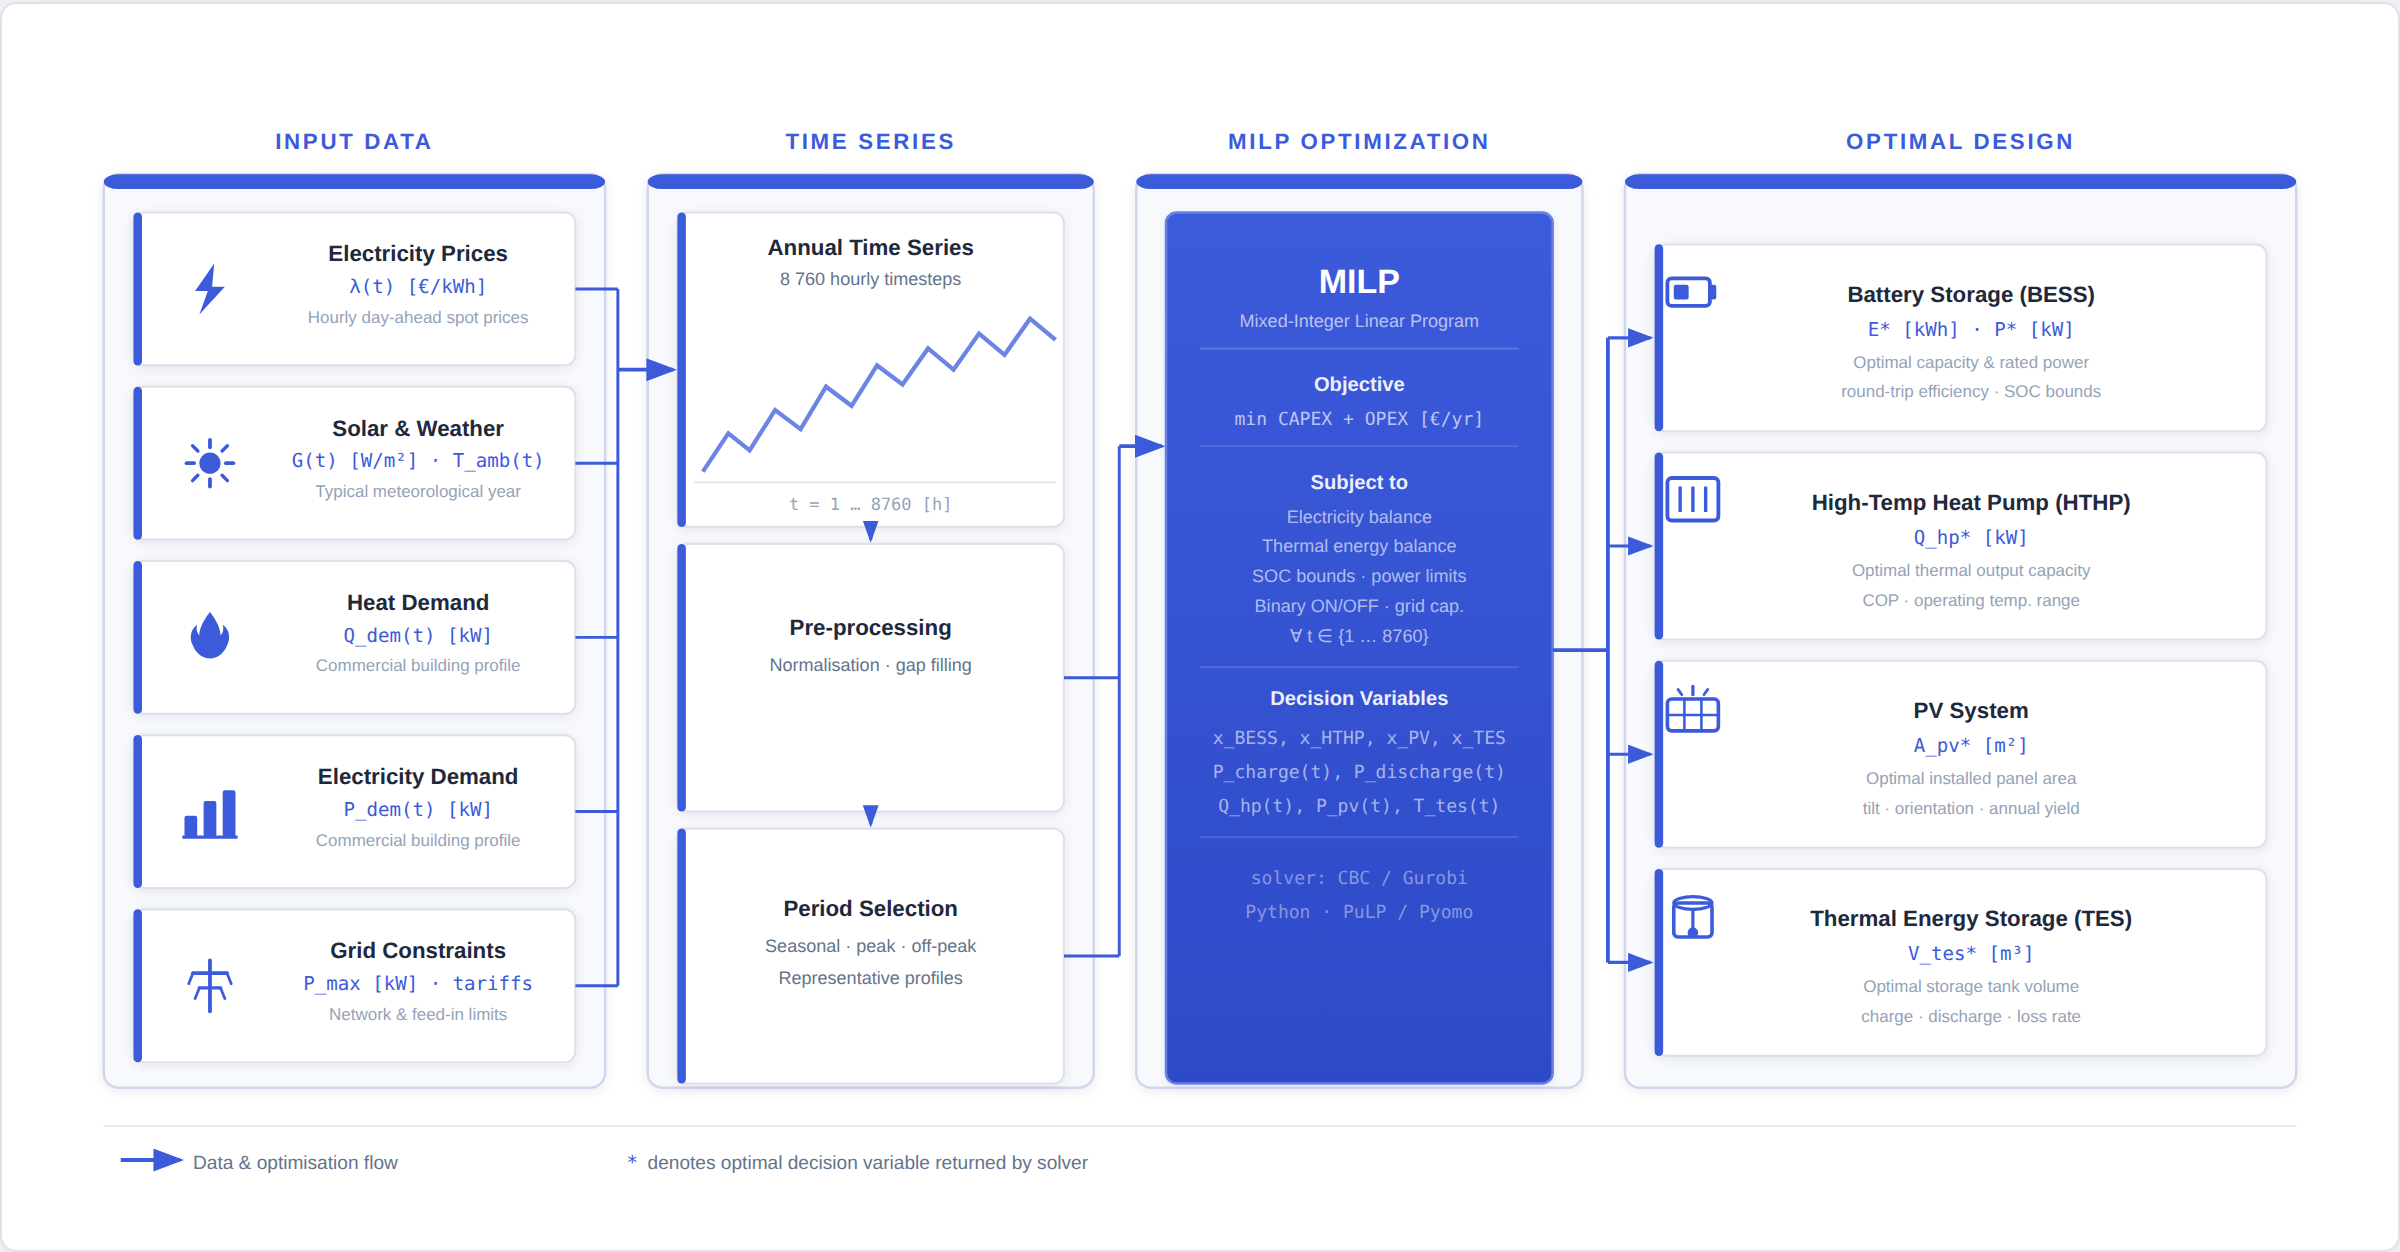
\includegraphics[width=\textwidth]{images/MILP_Methodology_Diagram.png}
    \caption{
        Overview of the proposed MILP-based design optimisation framework.
    }
    \label{fig:milp_methodology}
\end{figure}

The proposed design tool follows a four-stage workflow, illustrated in
\autoref{fig:milp_methodology}.
In the first stage, five hourly time-series datasets covering a full
calendar year (8\,760~time steps) are assembled:
day-ahead electricity spot prices~$\lambda(t)$~[\euro/kWh],
solar irradiation~$G(t)$~[W/m\textsuperscript{2}] and ambient
temperature~$T_\mathrm{amb}(t)$ derived from a typical meteorological
year~(TMY) file, the building's thermal heat demand~$Q_\mathrm{dem}(t)$~[kW],
its electrical demand~$P_\mathrm{dem}(t)$~[kW] (both representative of a
commercial building profile), and the applicable grid connection
constraints including the maximum import/export power~$P_\mathrm{max}$ and
network tariffs.

In the second stage the raw time series are normalised, validated, and
aligned to a common hourly resolution.
Representative operational periods (seasonal, peak, and off-peak) are
subsequently identified to characterise the building's energy-use pattern
throughout the year.

The third stage formulates a Mixed-Integer Linear Programme~(MILP).
The objective function minimises the total annualised system cost,
comprising capital expenditure~(CAPEX) and operational
expenditure~(OPEX):
%
\begin{equation}
    \min_{\mathbf{x},\,\mathbf{u}(t)}\;
    \mathrm{CAPEX}(\mathbf{x}) + \mathrm{OPEX}(\mathbf{u}(t))
    \label{eq:milp_obj}
\end{equation}
%
subject to the electricity and thermal energy balances,
state-of-charge~(SOC) bounds, component power limits,
binary on/off decisions, and grid capacity constraints,
enforced for every time step $t \in \{1,\ldots,8760\}$.
The programme is solved using an open-source Branch-and-Bound solver
(CBC) or the commercial solver Gurobi, implemented in Python via
PuLP~\cite{mitchell2011pulp} or Pyomo~\cite{hart2011pyomo},
with a relative optimality gap tolerance of~0.1\,\% and a time
limit of~3600\,s.

The fourth and final stage returns the cost-optimal installed
capacities of four storage and conversion technologies:
the BESS capacity~$E^*$~[kWh] and rated power~$P^*$~[kW],
the HTHP thermal output~$Q_\mathrm{hp}^*$~[kW],
the PV array area~$A_\mathrm{pv}^*$~[m\textsuperscript{2}],
and the TES tank volume~$V_\mathrm{tes}^*$~[m\textsuperscript{3}].

% ── ENERGY SYSTEM SCHEMATIC ──────────────────────────────────────
\begin{figure}[htbp]
    \centering
    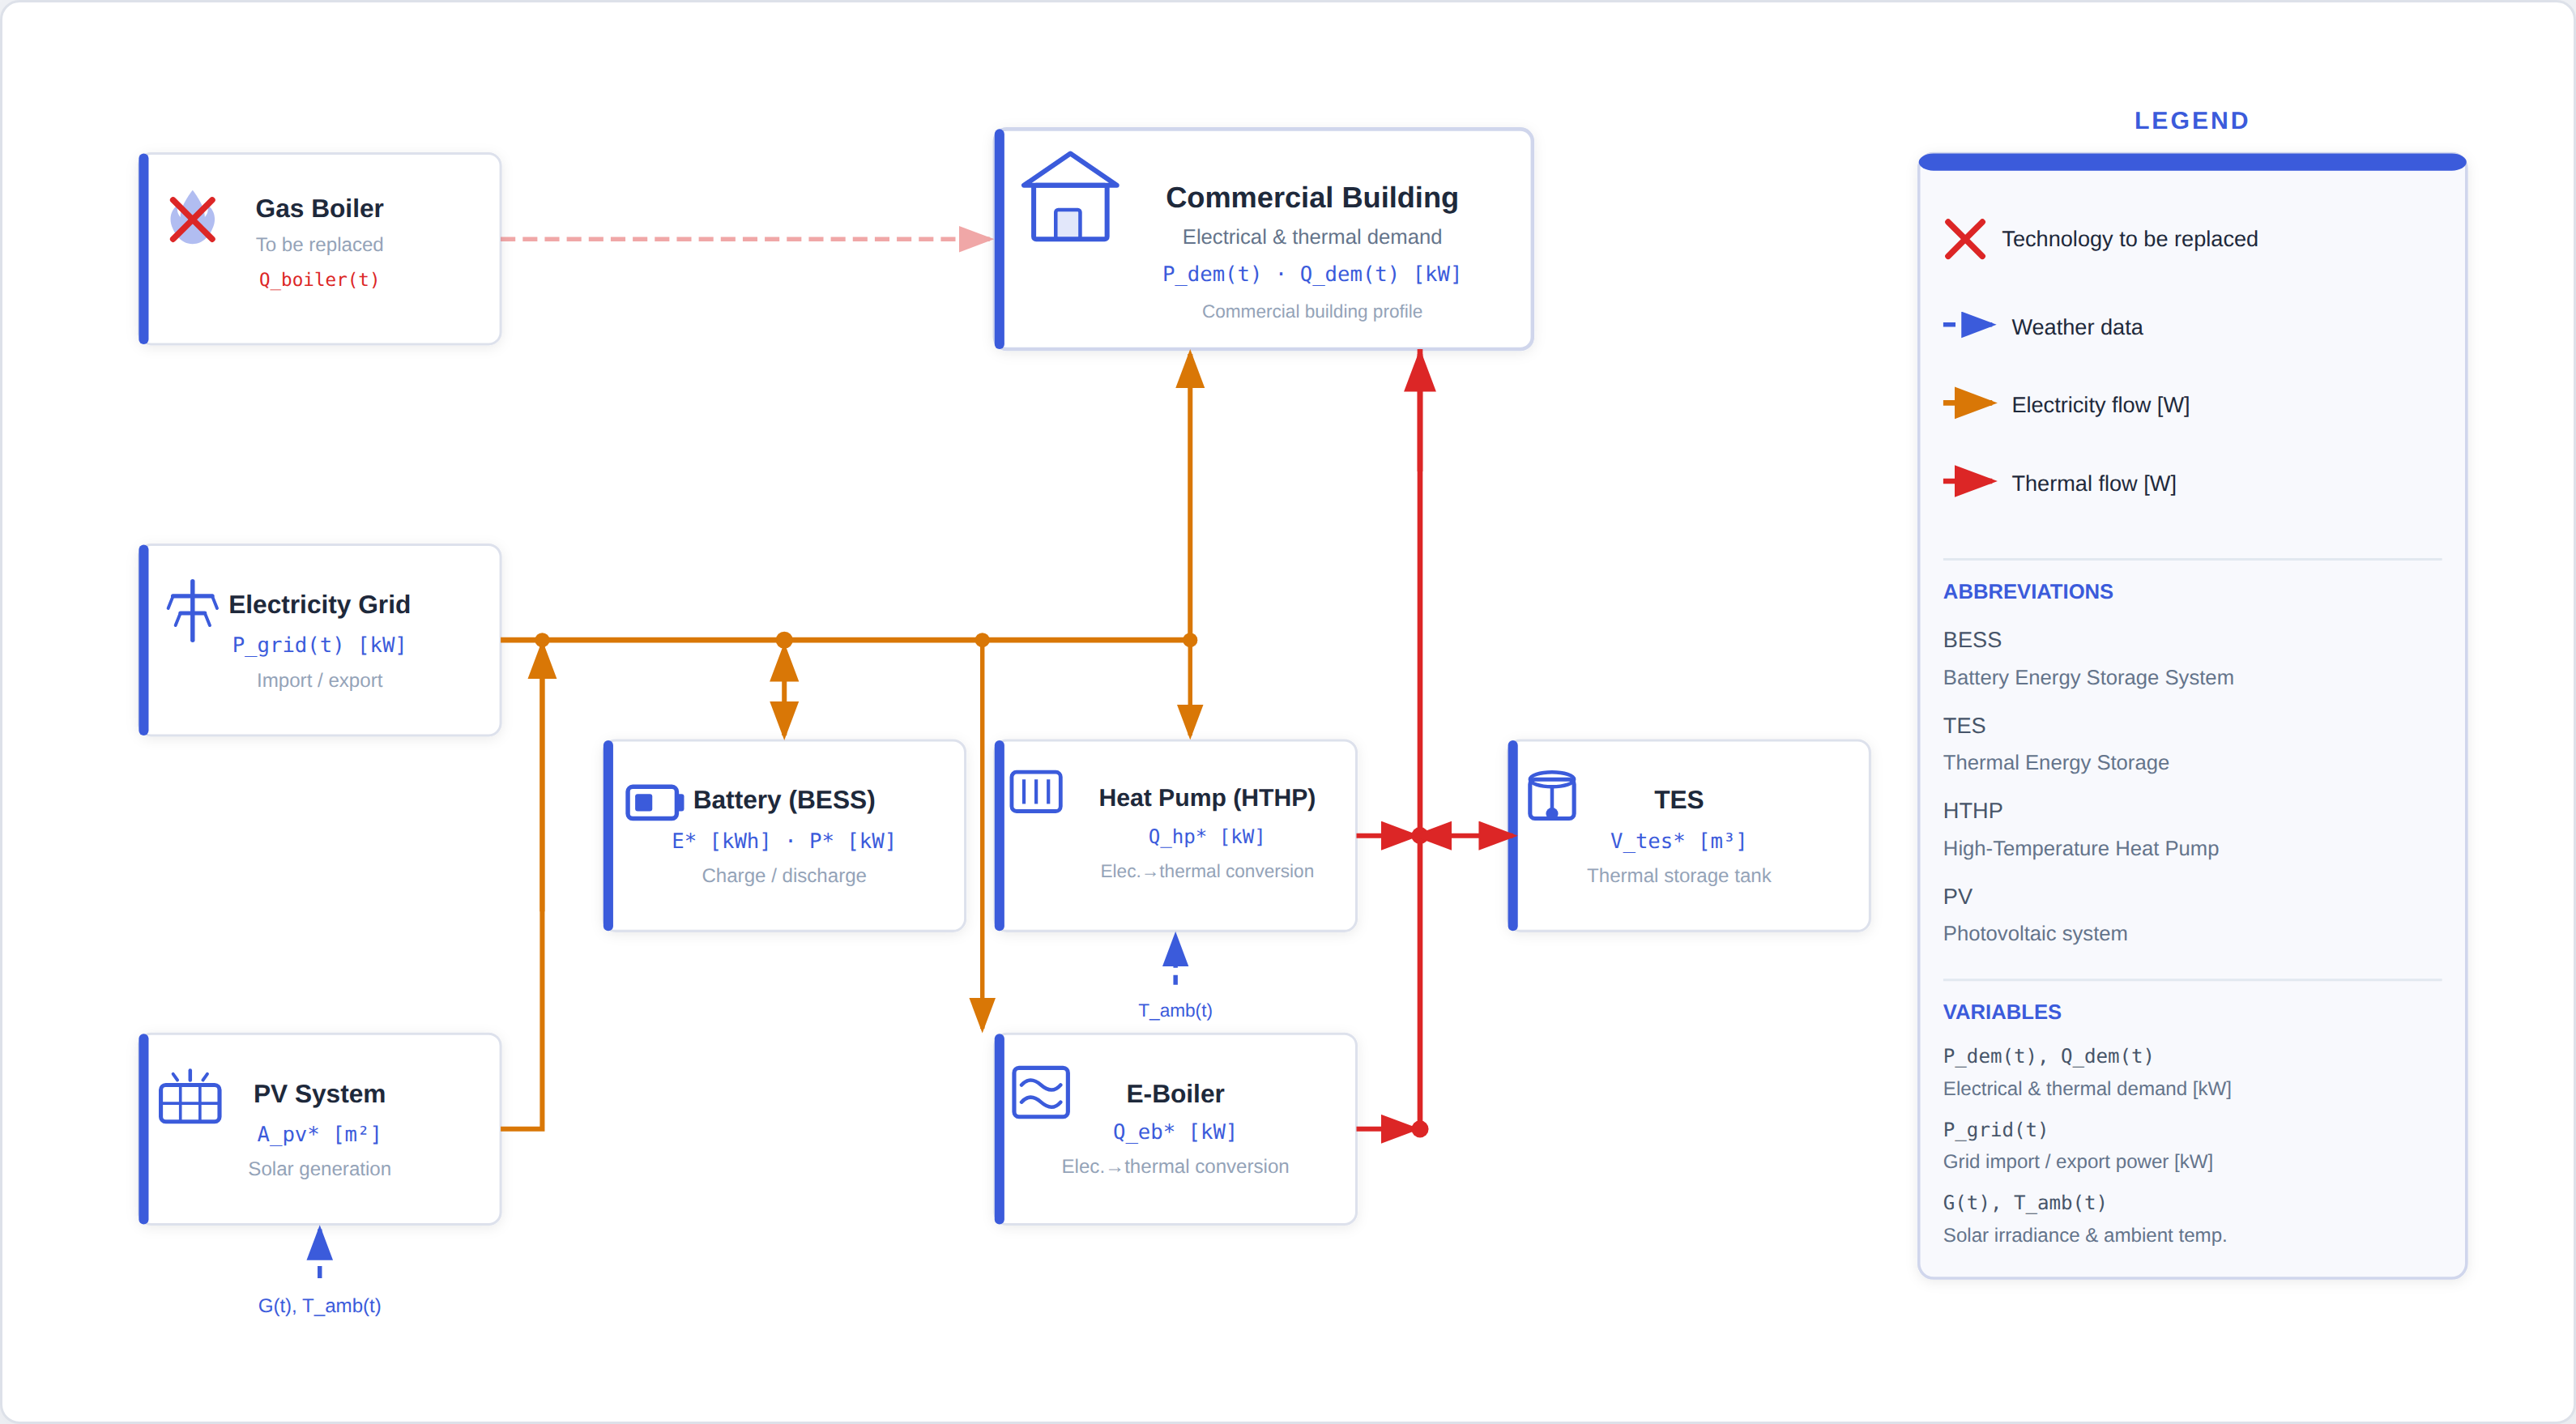
\includegraphics[width=\textwidth]{images/Energy_System_Schematic_final.png}
    \caption{
        Energy system schematic of the studied commercial building configuration,
        showing the electricity and thermal energy flows between all components.
        Dashed arrows indicate technologies to be replaced; solid orange arrows
        denote electricity flows; solid red arrows denote thermal flows.
    }
    \label{fig:energy_system}
\end{figure}

The energy system under study is depicted in \autoref{fig:energy_system}.
The commercial building is characterised by a simultaneous electrical demand
$P_\mathrm{dem}(t)$ and thermal heat demand $Q_\mathrm{dem}(t)$, both
resolved at an hourly resolution over a full calendar year.
Thermal supply is currently provided by a gas boiler
(supplying $Q_\mathrm{boiler}(t)$), which is designated for replacement by the
optimised system.

Four technologies constitute the candidate system.
On the electrical side, a photovoltaic~(PV) array of panel area
$A_\mathrm{pv}^*$~[m\textsuperscript{2}] generates power from incident solar
irradiation $G(t)$ at ambient temperature $T_\mathrm{amb}(t)$.
A Battery Energy Storage System~(BESS) with capacity $E^*$~[kWh] and rated
power $P^*$~[kW] enables temporal shifting of electrical energy through
charge and discharge cycles.
Residual electrical demand is balanced by import from, or export to, the
electricity grid at power $P_\mathrm{grid}(t)$~[kW], subject to the network
connection limits.

On the thermal side, a High-Temperature Heat Pump~(HTHP) converts electrical
energy into heat at a rated thermal output $Q_\mathrm{hp}^*$~[kW], with
performance characterised by its coefficient of performance~(COP) as a
function of $T_\mathrm{amb}(t)$.
An electric boiler~(E-Boiler) provides supplementary thermal output
$Q_\mathrm{eb}^*$~[kW] to cover peak demands or periods when the heat pump
alone is insufficient.
Thermal energy can be buffered in a Thermal Energy Storage~(TES) tank of
volume $V_\mathrm{tes}^*$~[m\textsuperscript{3}], decoupling heat generation
from instantaneous demand.
Together, these four technologies  BESS, HTHP, PV, and TES  form the
decision space of the MILP optimisation described in
\autoref{eq:milp_obj}, with their optimal capacities returned as the
primary output of the design tool

\section{Mixed-Integer Linear Programming (MILP)}
\label{sub:milp_advantages}

MILP is widely recognized in academic and industrial literature as the state-of-the-art methodology for optimizing the design and scheduling of energy systems\cite{Stinner2021ModelComplexity} \cite{Urbanucci2018Limits}.To understand the advantages of MILP, it is first necessary to understand the underlying computational mechanism used by modern solvers (e.g., Gurobi, CPLEX). 
\subsection{ MILP algorithm}




A \textbf{Mixed-Integer Linear Programming (MILP)} model is a mathematical optimization model where the objective function and all constraints are linear, but some, or all, of the decision variables are restricted to be integers (which can include binary, or 0-1, variables). The standard form of an MILP problem is:

\begin{equation}
\begin{aligned}
\text{Minimize (or Maximize)} \quad & \mathbf{c}^T\mathbf{x} + \mathbf{d}^T\mathbf{y} \\
\text{Subject to} \quad & \mathbf{A}\mathbf{x} + \mathbf{B}\mathbf{y} \le \mathbf{b} \\
& \mathbf{x} \ge 0, \quad \mathbf{x} \in \mathbb{R}^n \\
& \mathbf{y} \ge 0, \quad \mathbf{y} \in \mathbb{Z}^m
\end{aligned}
\end{equation}

Where:
\begin{itemize}
    \item $\mathbf{x}$ is a vector of \textbf{continuous} decision variables.
    \item $\mathbf{y}$ is a vector of \textbf{integer} decision variables (often binary variables are used to model yes/no decisions).
    \item $\mathbf{c}$ and $\mathbf{d}$ are vectors of coefficients for the objective function.
    \item $\mathbf{A}$ and $\mathbf{B}$ are matrices of coefficients for the constraints.
    \item $\mathbf{b}$ is a vector of right-hand side values for the constraints.
\end{itemize}

\section*{Key Components}

\begin{itemize}
    \item \textbf{Linear Objective Function:} The goal (e.g., minimizing cost or maximizing profit) is expressed as a linear combination of the variables. For example, \texttt{Minimize Cost = c1*x1 + c2*x2 + ...}.
    \item \textbf{Linear Constraints:} The limitations and requirements of the problem (e.g., resource availability, demand, capacity) are expressed as linear equations or inequalities. Non-linear expressions like \texttt{x1*x2} are not allowed, though some can be linearized using specific modeling techniques.
    \item \textbf{Mixed Variables:} The defining characteristic is the presence of both continuous variables (which can take any real value) and integer variables (which are restricted to whole numbers).
\end{itemize}


\section*{Solution Approach}

MILP problems are generally NP-hard and more difficult to solve than pure linear programming problems. Solvers (such as CPLEX, Gurobi, or SCIP) typically use algorithms like \textbf{Branch and Bound} or \textbf{Branch and Cut}. These methods work by:
\begin{enumerate}
    \item Solving a relaxed version of the problem (ignoring the integer constraints) to get a lower bound on the optimal solution.
    \item Systematically exploring a search tree (branching) and adding constraints (cutting planes) to find an optimal integer-feasible solution.
\end{enumerate}
\section*{Example}
\begin{figure}[h]
    \centering
    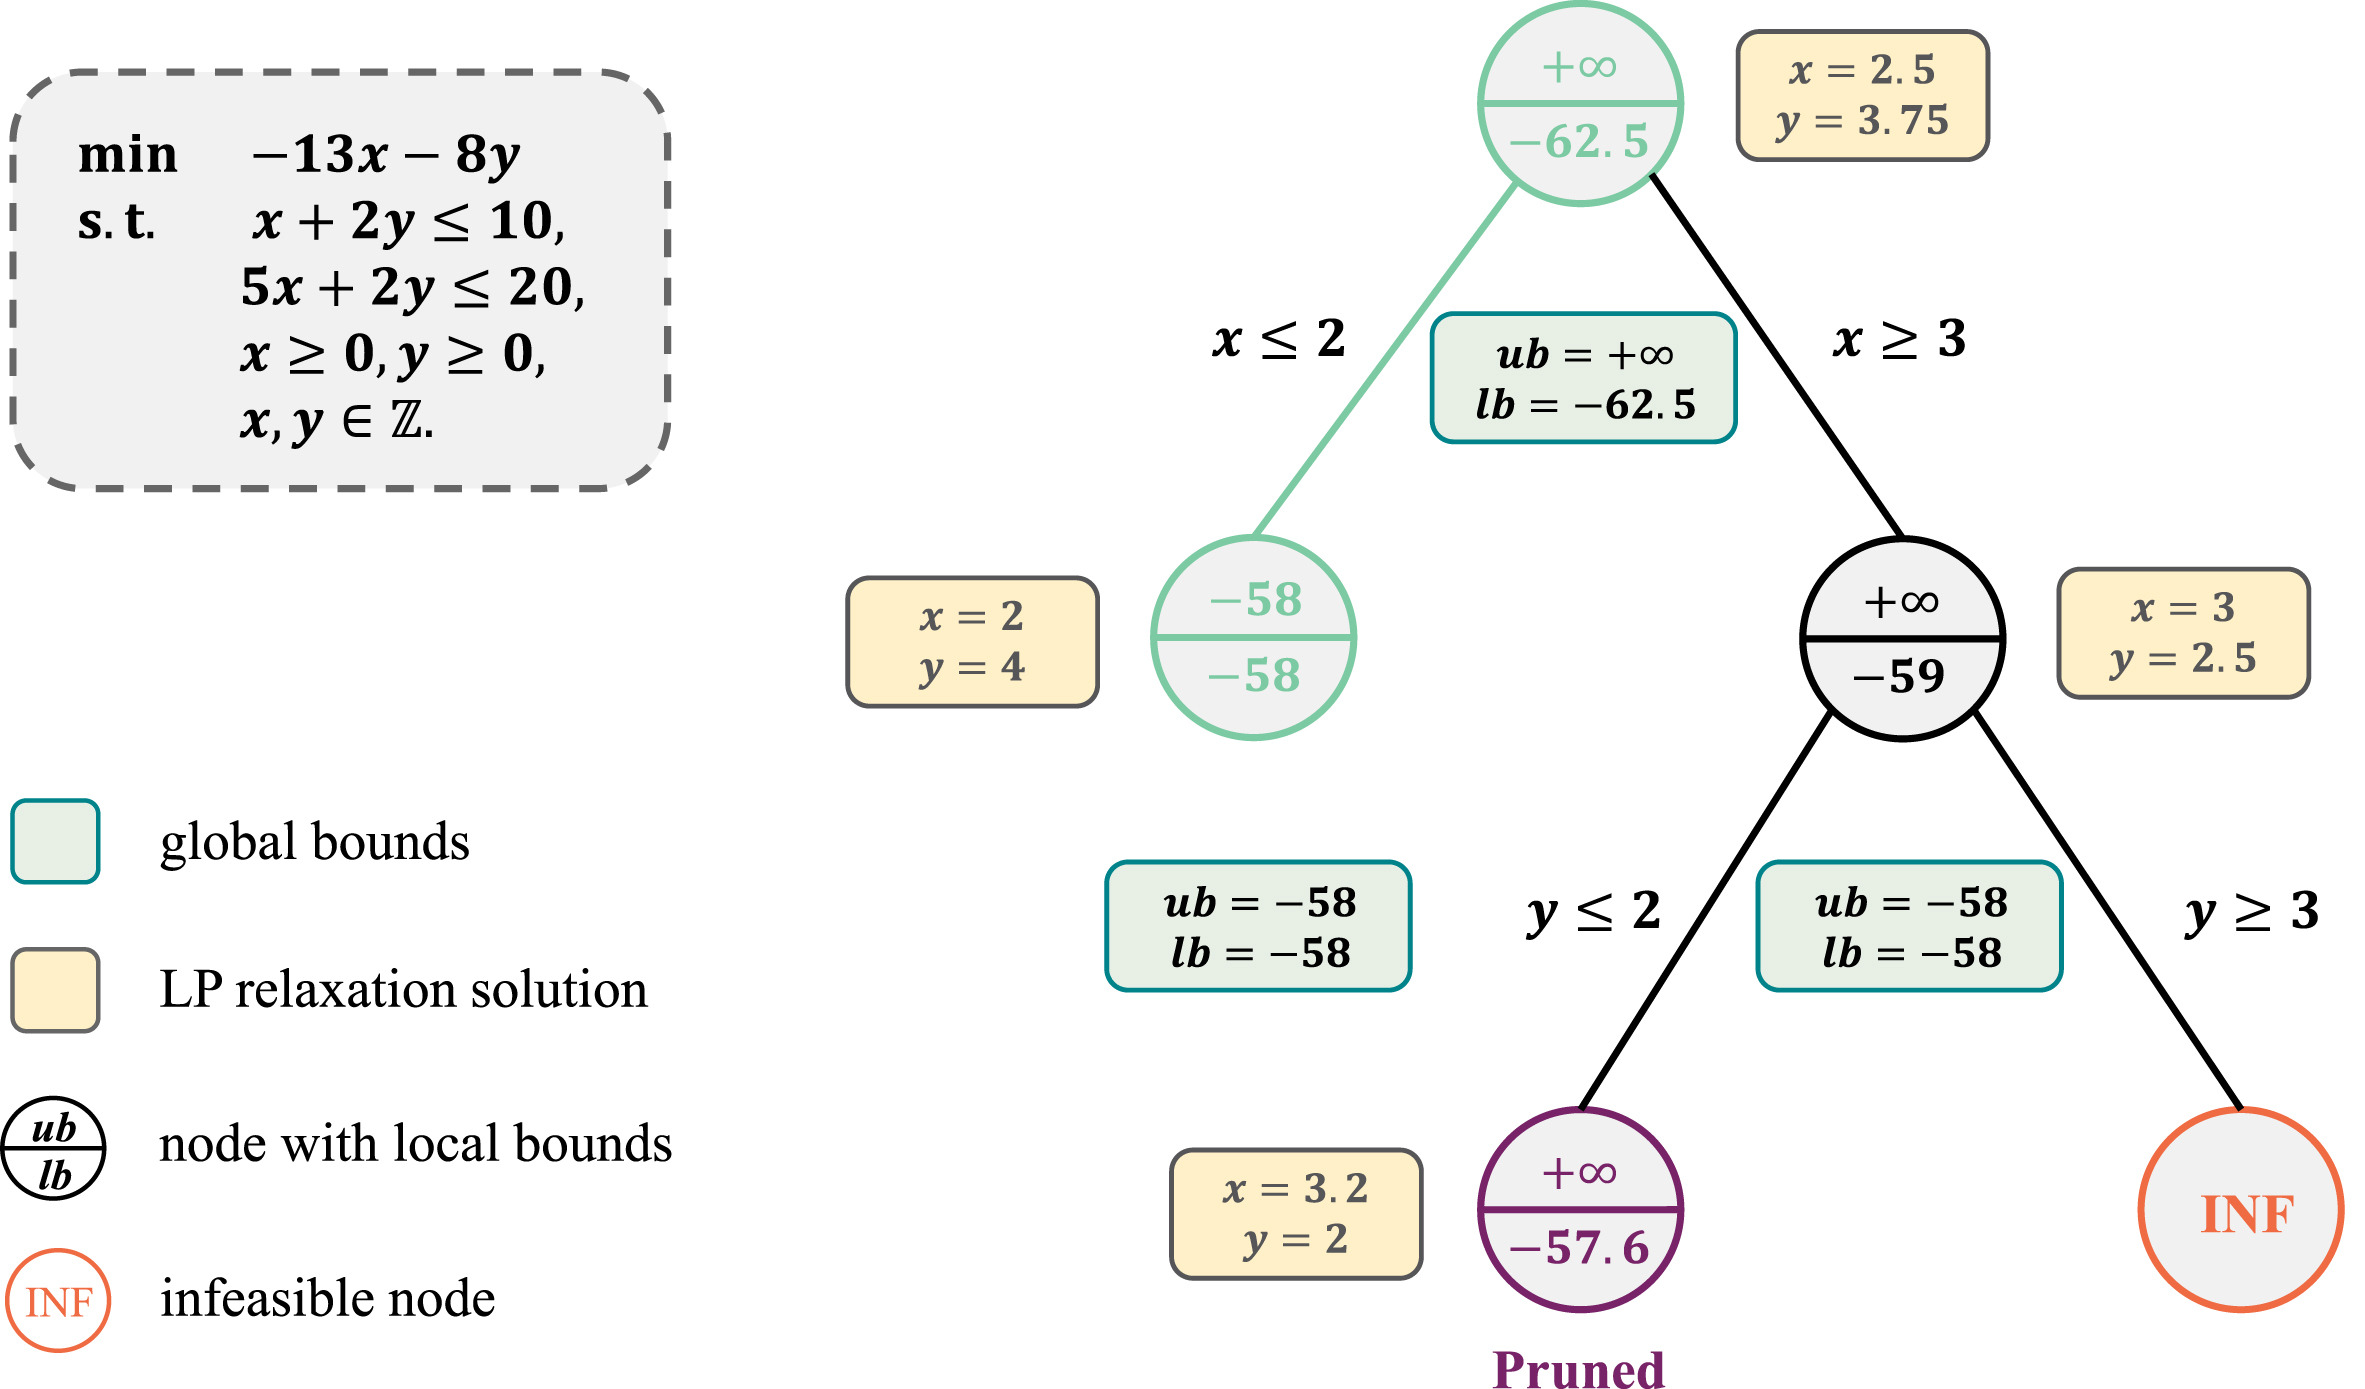
\includegraphics[width=0.8\textwidth]{images/milp_pic.jpg}
    \caption{Schematic of the Solution approach of MILP \cite{du2025learning}}
    \label{fig:example_image}
    
\end{figure}

\subsubsection{The Branching Decision (Example: PV Investment)}

Consider the binary variable for investing in PV system capacity, denoted $y_{\text{PV}} \in \{0, 1\}$.

\begin{itemize}
    \item \textbf{Initial Problem Node (Root Node):} $\min C_{\text{total}}$ with $0 \le y_{\text{PV}} \le 1$.
    \item \textbf{Branching Operation:} The solver partitions the original problem into two mutually exclusive subproblems:
\end{itemize}

\begin{align*}
    \text{Subproblem 1 (Assigned to Core 1):} \quad & \min C_{\text{total}} \\
    & \text{subject to } y_{\text{PV}} = 1 \quad (\text{PV is Purchased})
\end{align*}

\begin{align*}
    \text{Subproblem 2 (Assigned to Core 2):} \quad & \min C_{\text{total}} \\
    & \text{subject to } y_{\text{PV}} = 0 \quad (\text{PV is Not Purchased})
\end{align*}

\subsection{Parallel Processing and Pruning}

\begin{itemize}
    \item \textbf{Parallel Execution:} Core 1 searches for the best design \textit{assuming} PV is bought, while Core 2 searches for the best design \textit{assuming} PV is not bought.
    \item \textbf{Global Update:} If Core 1 quickly finds a feasible solution with total cost $\boldsymbol{C_{\text{Upper}} = \$10,000}$, this value is immediately broadcasted as the new \textbf{Global Upper Bound} on the final cost.
    \item \textbf{Pruning:} If Core 2 finds that the theoretical minimum cost in its branch (its Lower Bound) is $\boldsymbol{L_{\text{Subproblem 2}} = \$10,500}$, Core 2 can immediately \textbf{prune} its entire branch because it cannot contain a solution better than the already known $\boldsymbol{C_{\text{Upper}} = \$10,000}$.
\end{itemize}



\subsection{MILP advantages}
\subsubsection{Guarantee of Global Optimality}

As a deterministic mathematical programming technique, MILP is fundamentally designed to find the exact best possible outcome for a given objective function.
It guarantees finding a globally optimal solution when the problem converges \cite{Urbanucci2018Limits}, a critical advantage over heuristic methods (such as Genetic Algorithms or Particle Swarm Optimization), which can only guarantee finding acceptable solutions or local optima.

\subsubsection{Integration of Discrete and Continuous Decisions}

MILP is essential for system design and sizing because it effectively integrates the two necessary classes of variables:
\begin{itemize}
    \item \textbf{Integer/Binary Variables:} These are necessary to model structural and commitment decisions, such as the selection of a technology (e.g., using a Heat Pump or not), the existence of a component, the integer number of units to install, or the binary on/off status of a component at each time step.
    \item \textbf{Continuous Variables:} These model the operational schedule and energy flow, such as the electrical power being dispatched or the continuous volume of a storage unit.
\end{itemize}
This dual capability allows MILP to perform the required co-optimization of investment and operation simultaneously \cite{Bordin2020MILP}.

\subsubsection{Handling Non-Linearity via Linearization}

While the presence of complex, high-order non-linear models (e.g., in thermodynamics or equipment performance curves) presents a challenge, MILP addresses this through robust techniques.
The primary method is \textbf{Piecewise Linear (PWL) approximation}.
This technique simplifies non-linear functions (like the thermal dynamics of an Electric Water Heater or the variable efficiency of an inverter) into a series of linear segments.
By converting the problem into a strictly linear form, the overall optimization process can be performed by commercially available solvers (e.g., CPLEX, Gurobi) efficiently, providing an "efficiently solvable model" for these complex problems.
MILP's use of this technique is why it remains the preferred approach over complex Mixed-Integer Non-Linear Programming (MINLP) problems, which often have higher computational requirements \cite{Urbanucci2018Limits, Fuso2025University}.



\subsection{Optimization Objective Functions in MILP}

\subsection*{Cost Minimization (Economic)}

The minimization of total cost is the most common objective, aiming for the economically optimal design and operation.

\begin{itemize}
    \item \textbf{Objective:} Minimize Total Annual Cost ($C_{\text{total}}$) or Lifetime Cost.
    \item \textbf{Key Components:} Total costs comprise Investment Costs ($C_{\text{invest}}$) and Operational Costs ($C_{\text{op}}$).
    \begin{enumerate}
        \item \textbf{Investment Costs ($C_{\text{invest}}$):} The annualized cost is spread over the component's lifetime using an Annuity Factor (ANF). Non-linear cost functions are typically addressed by using discrete equipment sizes or linear approximations.
        $$C_{\text{invest}} = \sum_{i} ANF^{-1} \cdot (C_{\text{inv\_fix},i} + c_{\text{inv\_cap},i} \cdot cap_{i}^{m_{i}})$$
        \item \textbf{Operational Costs ($C_{\text{op}}$):} Includes energy costs (based on constant or variable electricity prices, e.g., time-of-use tariffs) and maintenance costs.
        $$ \min C_{\text{total}} = C_{\text{op}} + ANF^{-1} \cdot C_{\text{invest}} $$
    \end{enumerate}
\end{itemize}

\subsection*{CO$_2$ Emissions Minimization (Environmental)}

This objective focuses on reducing the system's environmental impact.

\begin{itemize}
    \item \textbf{Objective:} Minimize Total $\mathbf{CO_2}$ Emissions.
    \item \textbf{Key Components:} Emissions are calculated by weighing the consumption of electricity and other fuels by their respective $\mathbf{CO_2}$ emission factors. This often aims to shift electricity consumption to periods when the grid's carbon intensity is lower. Primary Energy Consumption (PEC) is sometimes used as a related metric.
\end{itemize}

\subsection*{Mathematical Formulation}

The overall objective function is the sum of operational and amortized embodied $\text{CO}_2$ emissions:
$$
\min \text{C}_{\text{CO}_2}^{\text{Total}} = \text{C}_{\text{CO}_2}^{\text{Op}} + \text{C}_{\text{CO}_2}^{\text{Emb}}
$$

\textbf{1. Operational Emissions ($\text{C}_{\text{CO}_2}^{\text{Op}}$) - Minimizing Grid Carbon Intensity}

\begin{equation}
\min \text{C}_{\text{CO}_2}^{\text{Op}} = \sum_{t \in T} \left( \sum_{i \in I} \text{E}_{\text{CO}_2,i,t}^{\text{Op}} \cdot \text{P}_{i,t}^{\text{Cons}} \cdot \Delta t \right)
\end{equation}

\subsection*{Multi-Criteria Optimization}

To balance conflicting objectives like cost minimization and Co2 emmisions minimization, multi-criteria optimization is applied.

\begin{itemize}
    \item \textbf{Approach:} The most common method is the \textbf{weighted summation method}, which combines normalized objectives into a single linear objective function using weighting factors ($\alpha$, $\beta$).
    \item \textbf{Weighted Sum Objective:}
    $$\min f = \alpha (\mu C) + \beta D$$
    where $C$ is the cost, $D$ is a discomfort index (or other non-cost objective), and $\alpha$ and $\beta$ ($\alpha + \beta = 1$) are the user's preference factors. $\mu$ is a scaling factor for normalization.
\end{itemize}

\subsection{ epsilon constrained method to create pareto front}

The $\epsilon$-constraint method is highly effective for visualizing the \textbf{trade-off} between two conflicting objectives in a \textbf{Mixed-Integer Linear Programming (MILP)} problem, such as minimizing the \textbf{Total Annual Cost} ($f_{\text{Cost}}$) and minimizing the \textbf{Total Life Cycle $\text{CO}_2$ Emissions} ($f_{\text{CO}_2}$).

\subsection*{$\epsilon$-Constraint Method in MILP for Cost vs. $\text{CO}_2$}

In this specific case, the Multi-Objective Problem (MOP) is to simultaneously minimize both $f_{\text{Cost}}$ and $f_{\text{CO}_2}$:
$$
\min \left[ f_{\text{Cost}}(\mathbf{x}), f_{\text{CO}_2}(\mathbf{x}) \right] \\
\text{s.t. } \mathbf{x} \in \mathcal{X}
$$

The solution vector $\mathbf{x}$ includes both continuous variables (e.g., operational energy flows $\text{P}_{i,t}$) and integer/binary variables (e.g., component sizing $\text{Z}_j$, on/off status $u(t)$).
The feasible region $\mathcal{X}$ is defined by constraints, such as:
\begin{enumerate}
    \item \textbf{Investment Constraints:} Component capacities ($\text{Z}_j$) are non-negative and often discrete (MILP is applicable for incorporating discrete decisions).
    \item \textbf{Energy Balance:} Supply must meet demand in every time step.
    \item \textbf{Physical Limits:} Component models (e.g., Heat Pump COP, TES energy balance) must be satisfied.
\end{enumerate}

\subsubsection*{1. Transformation to Single-Objective Problem (SOP)}

The $\epsilon$-constraint method selects one objective as the primary optimization target.
If we choose to \textbf{minimize Total Annual Cost} ($f_{\text{Cost}}$), the $\mathbf{CO_2}$ objective ($f_{\text{CO}_2}$) is converted into a constraint bounded by a user-defined threshold, $\epsilon_{\text{CO}_2}$ (the Greek letter $\epsilon$ gives the method its name).

The resulting $\mathbf{SOP}$ solved by the $\mathbf{MILP}$ solver is:
$$
\min f_{\text{Cost}}(\mathbf{x}) \\
\text{s.t. } f_{\text{CO}_2}(\mathbf{x}) \leq \epsilon_{\text{CO}_2} \\
\mathbf{x} \in \mathcal{X}
$$

\subsubsection*{2. Generating the Pareto Front (Trade-off Curve)}

The \textbf{Pareto front} the set of non-dominated solutions where no objective can be improved without worsening the other is generated by systematically varying $\epsilon_{\text{CO}_2}$ and solving the MILP for each step.

\begin{enumerate}
    \item \textbf{Determine $\mathbf{CO_2}$ Range (Boundary Solutions):}
    \begin{itemize}
        \item \textbf{Max $\mathbf{CO_2}$ / Min Cost Point:} Solve the MILP to \textbf{only} minimize $f_{\text{Cost}}$.
        \item The resulting total $\text{CO}_2$ emissions, $f_{\text{CO}_2}^{\max}$, defines the largest $\epsilon_{\text{CO}_2}$ needed.
        \item This solution usually involves the cheapest, but most $\text{CO}_2$-intensive technologies (e.g., large Auxiliary Heater, small Heat Pump, minimal storage).
        \item \textbf{Min $\mathbf{CO_2}$ / Max Cost Point:} Solve the MILP to \textbf{only} minimize $f_{\text{CO}_2}$.
        \item The resulting total $\text{CO}_2$ emissions, $f_{\text{CO}_2}^{\min}$, defines the most restrictive $\epsilon_{\text{CO}_2}$ limit (which might require the largest or most expensive set of components, e.g., large $\mathbf{PV}$ and \textbf{Battery}).
    \end{itemize}
    \item \textbf{Discretization:} The range $\left[ f_{\text{CO}_2}^{\min}, f_{\text{CO}_2}^{\max} \right]$ is divided into a discrete number of steps $N$.
    \item Each step defines a new, tighter $\epsilon_{\text{CO}_2}$ value.
    \item \textbf{Iteration and Output:} For each $\epsilon_{\text{CO}_2}$ step, the SOP is solved.
    \item The optimal annual cost $f_{\text{Cost}}^{*}$ is recorded.
\end{enumerate}

This yields a set of points $\left( f_{\text{CO}_2}, f_{\text{Cost}}^{*} \right)$, which when plotted, visually represents the \textbf{cost-optimal system design} for every level of \textbf{$\text{CO}_2$ reduction} desired.
The steepness of the curve indicates the marginal cost of achieving further environmental improvement.

\begin{figure}[h]
    \centering
    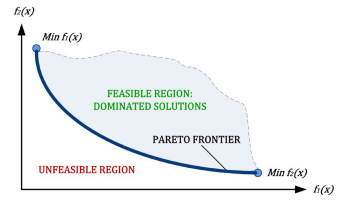
\includegraphics[width=0.8\textwidth]{images/pareto_Front.png}
    \caption{Schematic pareto Front\cite{PerezIribarren2023MILP}}
    \label{fig:example_image}
    
\end{figure}

\section{Component Modeling in Optimization Frameworks}
\label{sec:comp_modeling_methods}
\subsection{Component model requiremnts}
To be implemented within a Mixed-Integer Linear Programming (MILP) framework, a component model must fundamentally adhere to strict mathematical constraints regarding linearity to ensure the problem remains solvable by standard optimization algorithms~\cite{Krutzfeldt2021}.
Specifically, both the equality and inequality constraints defining the component's behavior, as well as the objective function, must be linear formulations involving real and integer decision variables~\cite{Wu2019}.
Since the actual thermodynamic dynamics of components such as the temperature-dependent Coefficient of Performance (COP) of heat pumps or the mixing processes in water heaters are inherently nonlinear and complex, they cannot be directly processed by MILP solvers~\cite{Wu2019, Krutzfeldt2021}.
Consequently, these models must undergo linearization or simplification, such as using piecewise linear approximation methods~\cite{Wu2019}, Taylor polynomial approximations~\cite{Krutzfeldt2021}, or simplifying thermal storage to a homogeneous capacity to avoid endogenous optimization problems~\cite{Steen2015}.
Furthermore, the physical system must be linearized temporally through time discretization, breaking continuous operations into distinct time steps to allow for the simultaneous optimization of design and operation~\cite{Krutzfeldt2021}.

\subsection{Lorentz Heat Pump Model Implementation} % Now a subsection
\label{sub:lorentz_model}

In energyPRO \cite{EMD_COP_HeatCapacity}, a simple \emph{Lorentz heat pump model} is implemented for calculating the theoretical Coefficient of Performance ($\text{COP}$). This model is based on the Carnot cycle, modified to account for the temperature variation during heat transfer by using mean temperatures.

\subsubsection{Theoretical COP Calculation} % Now a subsubsection

The theoretical $\text{COP}$ is calculated using the following thermodynamic relationship, where temperatures are expressed in Kelvin ($\text{K}$):

\[
\mathrm{COP} = \frac{T_{\mathrm{High,mean}}}{T_{\mathrm{High,mean}} - T_{\mathrm{Low,mean}}}
\]

\subsubsection{Mean Temperature of Delivered Hot Water ($T_{\mathrm{High,mean}}$)}

The mean temperature of the delivered hot water is computed using the logarithmic mean temperature over the condensor:

\[
T_{\mathrm{High,mean}} = 
\frac{T_{\mathrm{High,out}} - T_{\mathrm{High,in}}}
{\ln\!\left( \dfrac{T_{\mathrm{High,out}} + 273.15}{T_{\mathrm{High,in}} + 273.15} \right)}
\]

where:
\begin{itemize}
    \item $T_{\mathrm{High,out}}$ is the outlet water temperature (\textdegree C),
    \item $T_{\mathrm{High,in}}$ is the inlet water temperature (\textdegree C).
\end{itemize}

\subsubsection{Mean Temperature of the Heat Source ($T_{\mathrm{Low,mean}}$)}

\[
T_{\mathrm{Low,mean}} = 
\frac{T_{\mathrm{Low,out}} - T_{\mathrm{Low,in}}}
{\ln\!\left( \dfrac{T_{\mathrm{Low,out}} + 273.15}{T_{\mathrm{Low,in}} + 273.15} \right)}
\]

where:
\begin{itemize}
    \item $T_{\mathrm{Low,out}}$ is the initial temperature of the heat source (\textdegree C),
    \item $T_{\mathrm{Low,in}}$ is the cooled-down temperature of the heat source (\textdegree C).
\end{itemize}

\subsubsection{Actual COP and Heat Capacity Calculation}

The heat pump efficiency factor $\eta_{\mathrm{HP}}$ is computed from the stated COP and the theoretical COP under specification conditions (this efficiency can be derived from manufacturers data as in appendix \ref{appendix:datasheet_hthp}):

\[
\eta_{\mathrm{HP}} = 
\frac{\mathrm{COP}_{\mathrm{stated}}}{\mathrm{COP}_{\mathrm{theoretical,spec}}}
\]

At each timestep, the actual COP becomes:

\[
\mathrm{COP}_{\mathrm{actual}} = 
\mathrm{COP}_{\mathrm{theoretical,actual}} \cdot \eta_{\mathrm{HP}}
\]

The resulting heat capacity is:

\[
\dot{Q}_{\mathrm{heat}} = 
\mathrm{COP}_{\mathrm{actual}} \cdot \dot{E}_{\mathrm{elec}}
\]

\paragraph*{Limitation on Heat Capacity}




\subsection{Linearization for MILP:} 
When the $T_{\mathrm{High,out}}$ is considered a decision varible in the MILP optimization we cannot simply us the method desribed in \ref{sub:lorentz_model} we then need to linearize the equation
as done by Krutzefeldt et al. \cite{Germanbuiling}. The resulting non-linear energy relation $\left(P_{el} = Q_{HP} / COP\right)$ is transformed into a linear constraint by applying a multi-dimensional \textbf{Taylor polynomial approximation} around a fixed operation point (OP). The linear approximation $f(x) \approx f(a) + \nabla f(a) \cdot (x-a)$ for the electric power $P_{el, HP, t}$ (function $f$) with state vector $x = (\dot{Q}_{HP, t}, COP_{ t})$ and fixed operation point $a = (\dot{Q}_{OP}, COP_{OP})$ yields the constraint:
\begin{equation}
\begin{split}
\label{eq:taylor}
P_{el,HP,t} = &\frac{\dot{Q}_{OP}}{COP_{OP}} + \frac{1}{COP_{OP}} \cdot (\dot{Q}_{HP,t} - \dot{Q}_{OP}) \\
&- \frac{\dot{Q}_{OP}}{COP_{OP}^{2}} \cdot (COP_{t} - COP_{OP})
\end{split}
\end{equation}
This process enables the inclusion of realistic, state-dependent COP in the MILP model while maintaining linearity. Note that this approach is only needed when het COP contains a decision variable that is used in MILP, only then the equation $\left(P_{el} = Q_{HP} / COP\right)$ is non-linear( in the decision variables). In this master thesis we assume $T_{\mathrm{High,out}}$ as a given so we can use the method as described in \ref{sub:lorentz_model}.

\subsection{Thermal Energy Storage (TES) Modeling}

\subsubsection{Thermal Energy Storage (TES) Technology Selection}

Thermal Energy Storage (TES) systems can be implemented using several distinct technologies, each offering a different trade-off between volumetric energy density, cost, complexity, and operating temperature range. The three most relevant categories for building-scale applications are sensible heat storage (typically water tanks), latent heat storage (Phase Change Materials, PCM), and thermochemical storage.

\textbf{Sensible heat storage} using water tanks is the most mature and widely deployed technology. Water has a high specific heat capacity ($c_p \approx 4.18\,\text{kJ/kg·K}$), is inexpensive, non-toxic, and compatible with a broad range of heating and cooling systems. However, the volumetric energy density is relatively low: storing a meaningful quantity of thermal energy requires large tank volumes, which can be a limiting factor in space-constrained commercial building contexts \cite{Dincer2018}. Water tanks are typically operated between 40\,°C and 95\,°C for heating applications and are well-suited to coupling with high-temperature heat pumps (HTHPs).

\textbf{Latent heat storage} using Phase Change Materials (PCMs) exploits the energy absorbed or released during a phase transition (typically solid-to-liquid). PCMs can achieve volumetric energy densities 5--14 times higher than water for the same temperature lift, depending on the material selected \cite{Sharma2009}. This significantly reduced footprint makes LTES particularly attractive when available installation space is limited. The primary drawbacks are higher material and encapsulation costs, lower thermal conductivity (requiring enhanced heat exchanger designs), and sensitivity to the operating temperature window of the phase transition, which must be aligned with the supply temperature of the coupled heat source or sink \cite{Cabeza2014}. For HTHP-coupled systems, PCMs with melting points in the range of 55--80\,°C, such as fatty acids or paraffin waxes, are typically considered.

\textbf{Thermochemical storage} offers the highest theoretical energy density but remains largely at the research and pilot scale, with limited commercial availability and significant engineering complexity. It is therefore not considered further in this work.

A comparative summary of the relevant TES technologies is provided in Table~\ref{tab:tes_comparison}.

\begin{table}[h]
\centering
\caption{Comparative overview of TES technologies considered for HTHP-coupled building applications.}
\label{tab:tes_comparison}
\begin{tabular}{lccc}
\hline
\textbf{Property} & \textbf{Water tank} & \textbf{PCM (LTES)} & \textbf{Thermochemical} \\
\hline
Volumetric energy density & Low & Medium--High & Very High \\
Capital cost & Low & Medium--High & High \\
Technology readiness & High & Medium & Low \\
Required volume & High & Low--Medium & Very Low \\
Thermal conductivity & High & Low & Variable \\
Temperature flexibility & High & Narrow window & High \\
\hline
\end{tabular}
\end{table}

\subsubsection*{Selected Technology and Volume Constraint}

Given the space constraints typical of commercial building retrofits, this work models \textbf{Latent Thermal Energy Storage (LTES)} as the primary TES technology when there is limited space available. Its higher volumetric energy density allows more thermal capacity to be installed within the available footprint, making it well-suited for situations where installation space is a binding constraint.

To capture this spatial limitation within the optimization, the MILP model incorporates an optional maximum volume constraint on the TES unit:

\begin{equation}
    V_{\text{TES}} \leq V_{\text{TES,max}}
\end{equation}

\noindent where $V_{\text{TES}}$ [m$^3$] is the optimally determined storage volume and $V_{\text{TES,max}}$ [m$^3$] is a user-defined upper bound reflecting the physical space available at the installation site. When no space restriction applies, $V_{\text{TES,max}}$ can be set to an arbitrarily large value, leaving the optimizer free to select the cost-optimal storage capacity. Conversely, setting $V_{\text{TES,max}}$ to a finite value forces the MILP algorithm to respect the spatial constraint during sizing, potentially shifting the optimal solution toward more aggressive peak shaving via the HTHP or BESS rather than thermal storage.




The proposed optimization framework utilizes a linear model for thewater Thermal Energy Storage (TES) unit, representing a simplified or ideal stratified storage to maintain the tractability of the Mixed-Integer Linear Programming (MILP) problem \cite{Krien2020oemofsolph}. This approach balances accuracy with computational speed, as the detailed modeling of stratification, though more physically precise, significantly increases computation time. Studies show that the simplified model is often sufficiently accurate for operation optimization, as model overestimations and underestimations of temperature changes tend to compensate for each other, thus ensuring thermal comfort constraints are met \cite{Germanbuiling}.

The selection of a TES model for a Mixed-Integer Linear Programming (MILP) optimization tool involves a trade-off between \textbf{computational tractability} (simplicity) and \textbf{physical accuracy} (complexity) \cite{Krien2020oemofsolph}. The chosen model must accurately reflect real-world constraints, especially when coupled with temperature-sensitive technologies like Heat Pumps (HPs).



\subsubsection{Rule-of-Thumb Dimensioning}
In conventional planning, sizing the TES often relies on a \textbf{rule of thumb} to ensure reliability:
\begin{itemize}
    \item \textbf{Principle:} The storage should be able to provide its \textbf{peak thermal power} for a fixed duration, typically \textbf{6 to 7 hours} \cite{Krien2020oemofsolph}. This method is mainly used for preliminary heuristic sizing within the overall MILP design.
\end{itemize}

\subsubsection{Constant (Size-Independent) Losses}
For basic MILP operational models, thermal losses ($\dot{E}_{\text{loss}}$) can be simplified to be either neglected or represented by a \textbf{constant factor ($\delta$)} that is independent ofthe physical size ($Q_{\text{N}}$) \cite{Krien2020oemofsolph}.

\begin{equation}
Q_{t} = Q_{t-1}  - \delta + \dot{Q}_{\text{in},t} \eta_{\text{in}} \Delta t - \frac{\dot{Q}_{\text{out},t}}{\eta_{\text{out}}} \Delta t,
\label{eq:storage-simplified}
\end{equation}
with
\begin{align*}
\delta &= U (2 *\frac{\pi d^{2}}{4}+ \pi d h) \left(\Delta T_{\text{H0}} + \Delta T_{\text{C0}}\right)/2
\end{align*}

\begin{itemize}
    \item \textbf{Energy Balance:} This approach uses the core energy balance equation, but simplifies the loss terms to depend minimally on dynamic state or size \cite{1.5}.
    \item \textbf{Rationale:} This maintains strict linearity and computational speed, though it is the least physically accurate, as actual losses depend heavily on the temperature differential with the ambient environment.
\end{itemize}

\subsubsection{Stratified Thermal Storage (STS) 2-Zone Model}
The model implements a simplified \textbf{2-zone-model} of a large-scale sensible heat storage with ideal stratification for energy system optimization (see Figure 1 \cite{Krien2020oemofsolph}). This model assumes a cylindrical storage of diameter $d$ and height $h$ containing two perfectly separated bodies of water: a hot zone ($T_{\text{H}}$) and a cold zone ($T_{\text{C}}$). The temperatures are fixed to the feed-in/return temperatures of the heating system. When charging/discharging, the thermocline moves up or down. For investment problems, the diameter is typically fixed, and the height is adjusted to maintain linearity in the capacity calculation \cite{Krien2020oemofsolph}.


\begin{figure}[H]
    \centering
    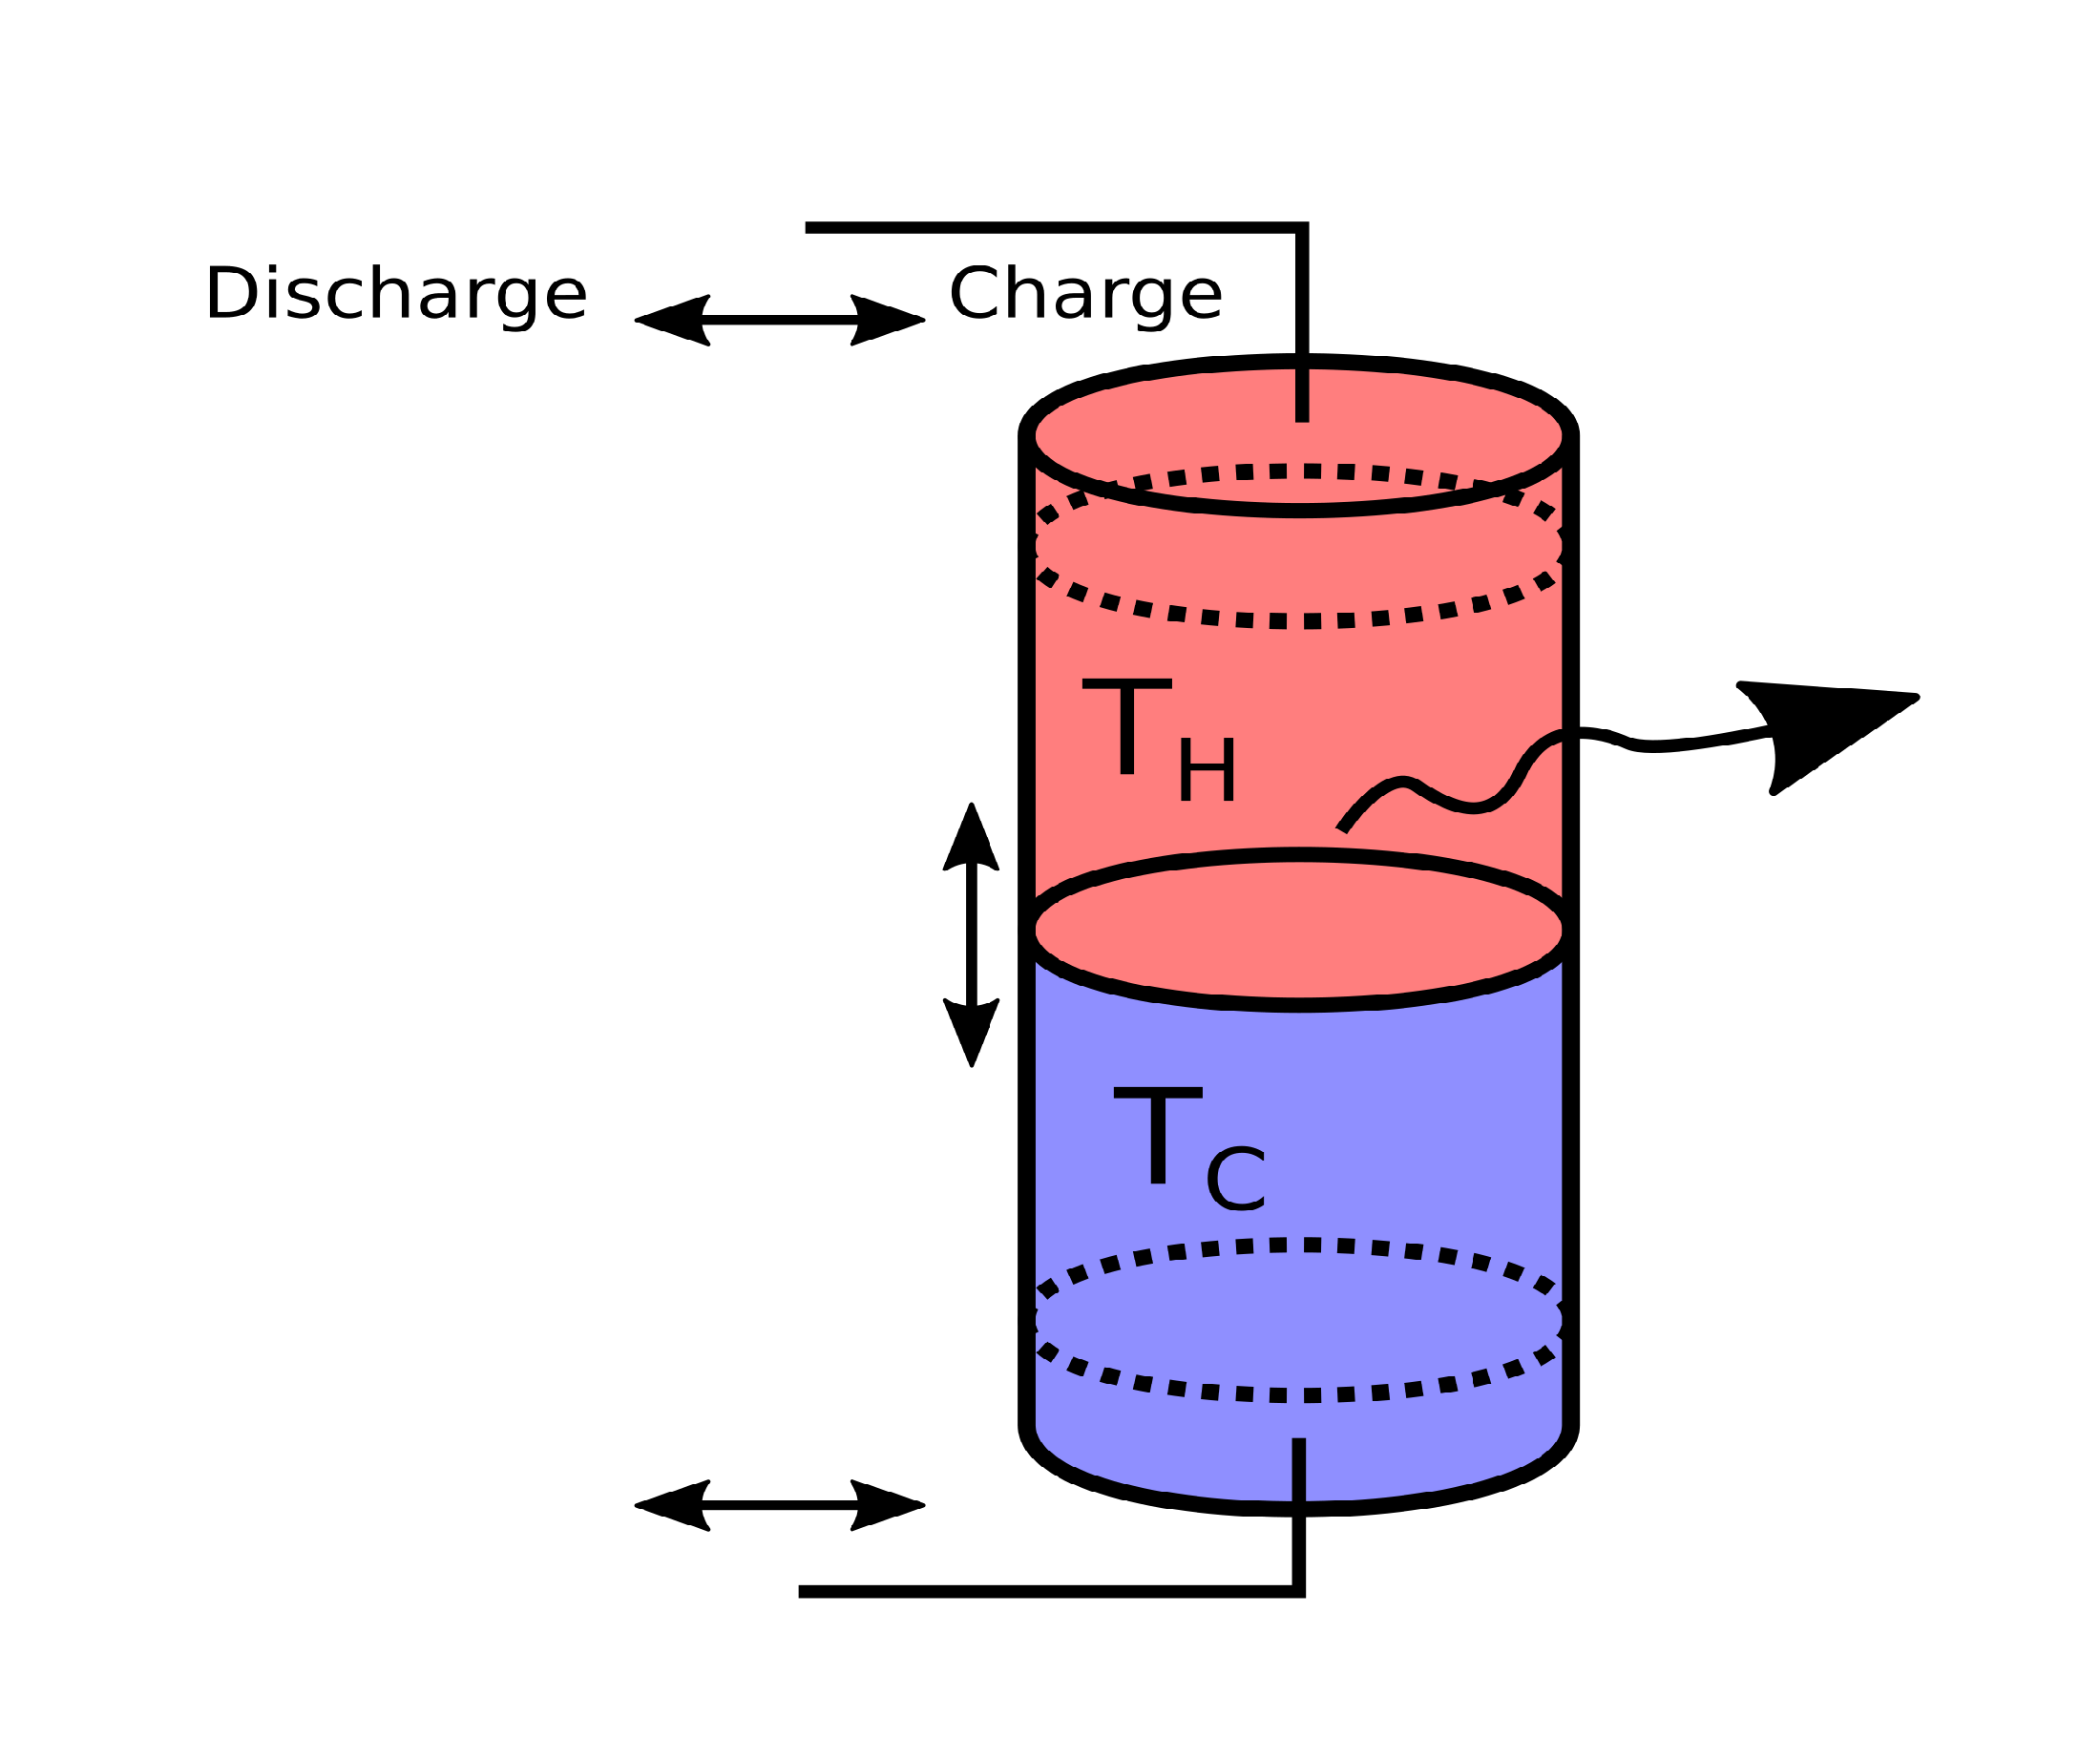
\includegraphics[width=0.4\textwidth]{images/TES_picture.png}
    \caption{Schematic of the simplified 2-zone model of a stratified thermal storage with constant hot ($T_{\text{H}}$) and cold ($T_{\text{C}}$) temperature regions \cite{Krien2020oemofsolph}.}
    \label{fig:stratifiedtes}
\end{figure}


\subsubsection{Energy Balance}

The equation describing the storage content at time step $t$ is the following:

\begin{equation}
Q_{t} = Q_{t-1} (1 - \beta) - \gamma Q_{\text{N}} - \delta + \dot{Q}_{\text{in},t} \eta_{\text{in}} \Delta t - \frac{\dot{Q}_{\text{out},t}}{\eta_{\text{out}}} \Delta t,
\label{eq:storage-stratified}
\end{equation}
with
\begin{align*}
Q_{N} &= \rho V c \Delta T_{\text{HC}} \\
V &= \frac{\pi d^{2}}{4} h \\
\beta &= U \frac{4}{d \rho c} \Delta t \\
\gamma &= U \frac{4}{d \rho c \Delta T_{\text{HC}}} \Delta T_{\text{C0}} \\
\delta &= U \frac{\pi d^{2}}{4} \left(\Delta T_{\text{H0}} + \Delta T_{\text{C0}}\right) \\
U &= \left( \frac{1}{\alpha_{\text{in}}} + \frac{t_{\text{isolation}}}{\lambda_{\text{isolation}}} + \frac{1}{\alpha_{\text{out}}} \right)^{-1}
\end{align*}

The three terms represent:
\begin{itemize}
    \item $\delta$: Constant heat losses through the top and bottom surfaces.
    \item $\gamma \cdot Q_{\text{N}}$: Losses through the total lateral surface assuming the storage to be empty (storage is at $T_{\text{C}}$, and $\Delta T_{\text{C0}}$ is the driving temperature difference), dependent on the height of the storage.
    \item $\beta \cdot Q_{t-1}$: Additional losses through the lateral surface that belong to the hot part of the water body, dependent on the state of charge.
\end{itemize}



The diameter $d$ is given and the height can be adapted to adapt the nominal capacity of the storage. With this assumption,\textbf{ all relations stay linear}.

Because of the space that diffuser plates for charging/discharging take up, it is assumed that the storage can neither be fully charged nor discharged, which is parametrised as a minimal/maximal storage level (indicated by the dotted lines in \ref{fig:stratifiedtes}).



\subsubsection{Capacity and Boundary Constraints}
The model is constrained by the physical capacity of the storage and boundary conditions required for optimization:

\begin{itemize}
\item \textbf{Cycle Constraint:} To model continuous operation, such as in a rolling horizon or repeated operation schedule, the stored energy at the last time step ($t_{\text{last}}$) must equal the stored energy at the initial time step ($t_{\text{zero}}$) of the \textbf{full} simulation.
 \begin{equation}
 Q_{t-1} = Q_{t}
\tag{10}
 \end{equation}

\item \textbf{Capacity Limit:} The instantaneous stored energy is bound by the nominal capacity to ensure physical realism.
\begin{equation}
0 \le Q_{t} \le Q_N
 \tag{11}
 \end{equation}
\end{itemize}

\vspace{0.5cm}

The use of this simplified model is advantageous for design and operational optimization due to its robustness and linearity within the MILP framework.
\subsubsection{ Comparison simple thermal storage vs stratified thermal storage}
\begin{figure}[H]
    \centering
    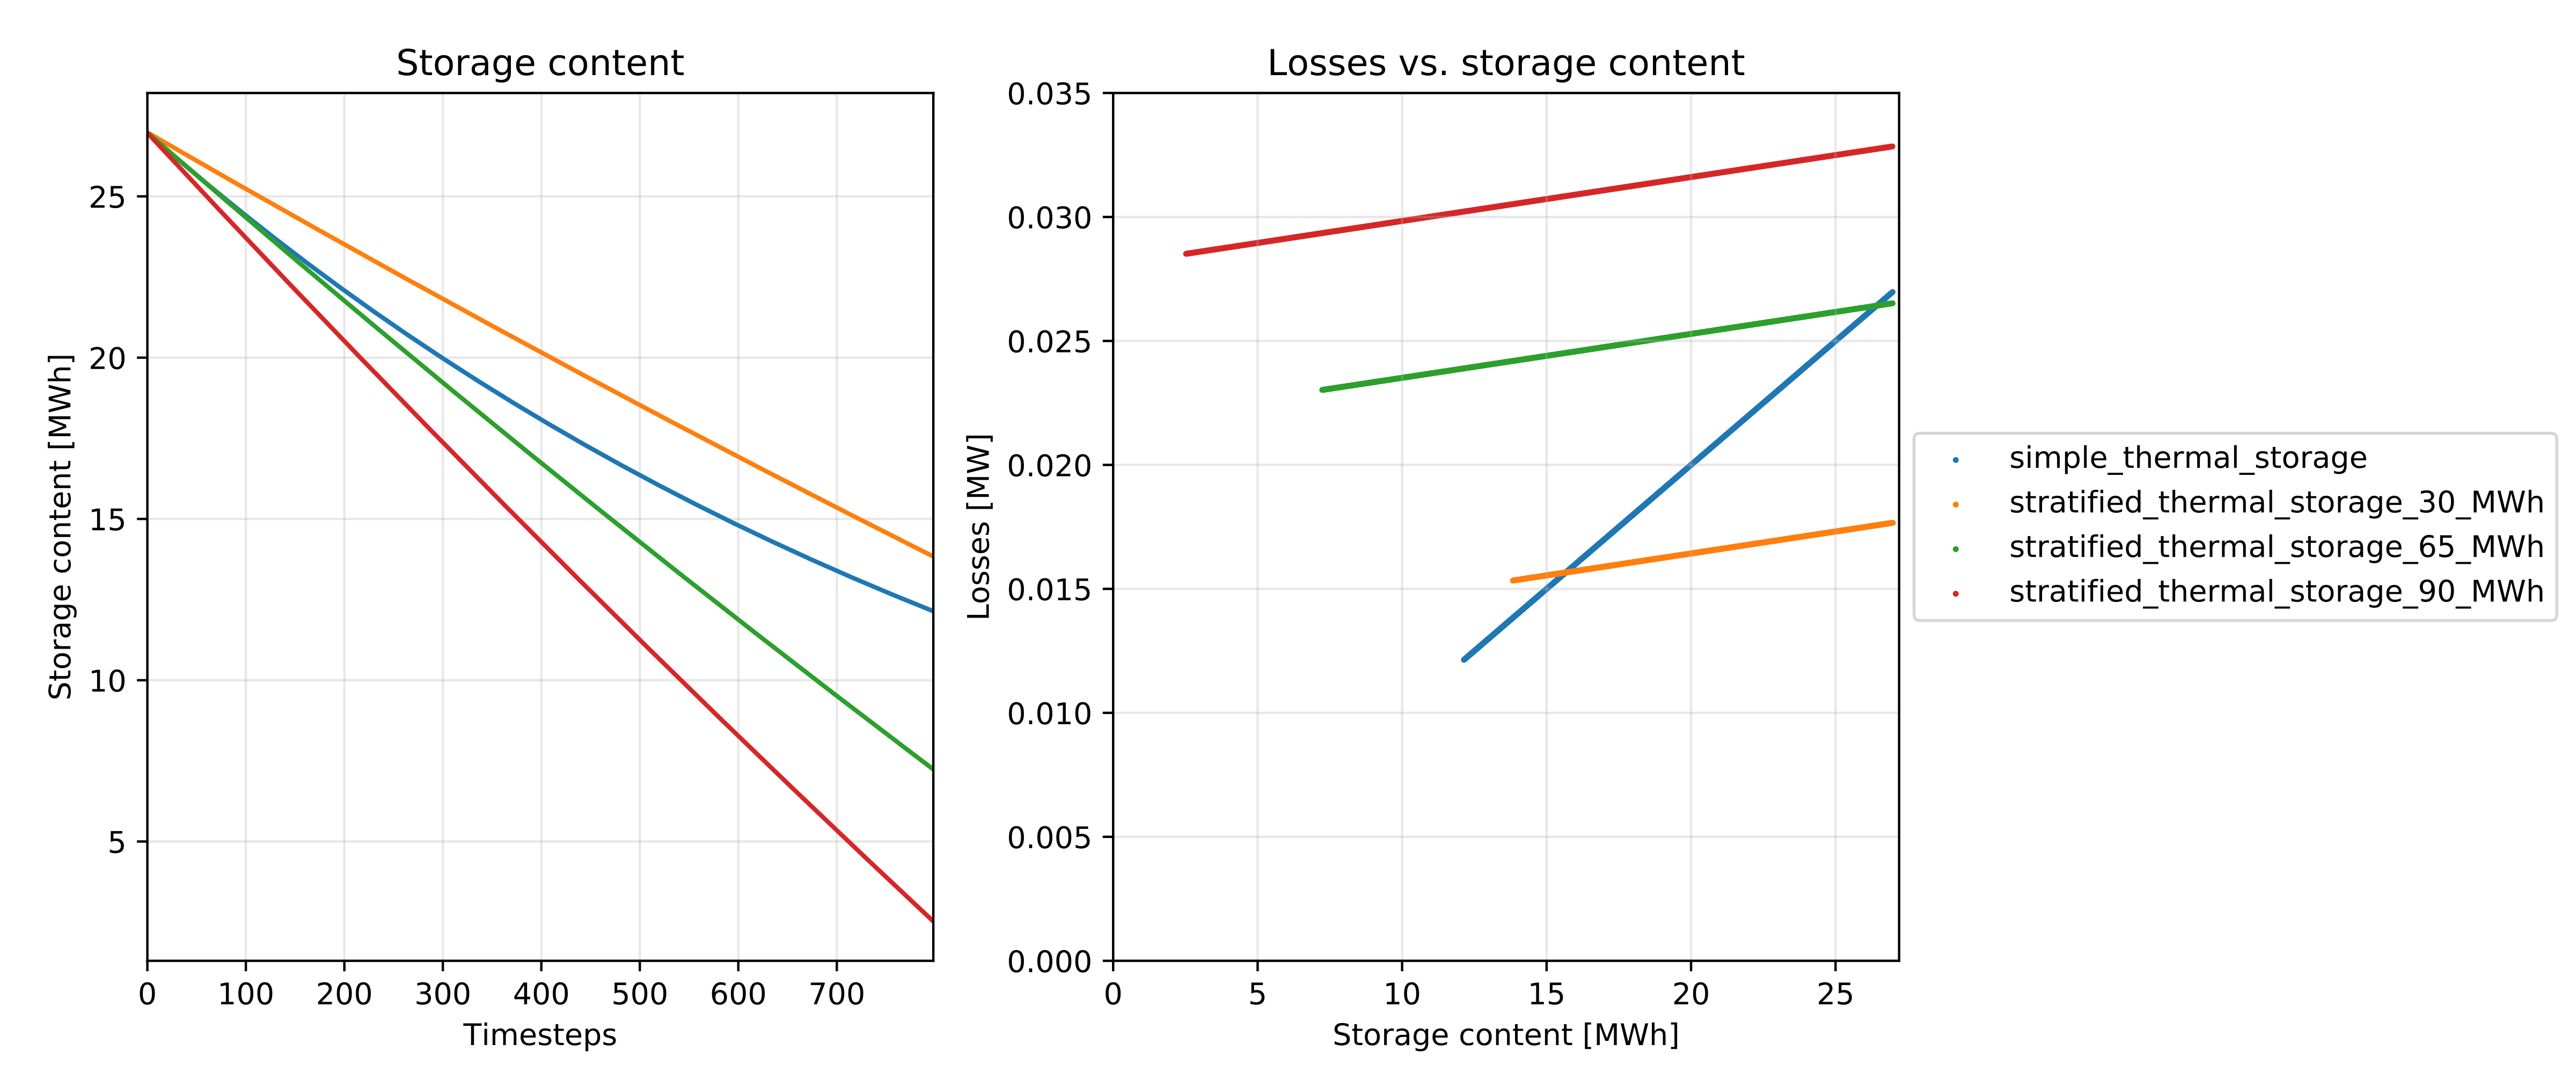
\includegraphics[width=\textwidth]{images/TES_simpleVScomplicated.png}
    \caption{Comparison of storage content decay over time (left) and heat losses versus actual storage content (right) for a simple thermal storage model and stratified thermal storage models of different nominal capacities (30 MWh, 65 MWh, and 90 MWh) \cite{Krien2020oemofsolph}.}
    \label{fig:storage_comparison}
\end{figure}

\ref{fig:storage_comparison} shows that the simpler TES models neglects the dependence of thermal losses on storage tank size, justifying the choice of the (slightly more complicated) stratified approach for our work.
The evident difference in both the absolute loss calculation and the decay of stored energy confirms that the \textbf{simple model is inadequate} for accurately simulating the TES unit's performance, especially for applications like heat pump coupling where temperature and heat loss dependency are critical for economic optimization \cite{Germanbuiling}. Therefore, the \textbf{stratified model is chosen} to ensure the MILP predictions are grounded in realistic thermal dynamics \cite{Germanbuiling}.


\subsection{Photovoltaic (PV) System modeling}

The electrical energy generated by the photovoltaic (PV) system is a crucial input for the overall Mixed-Integer Linear Programming (MILP) optimization framework. For the sake of generality, the PV generation is modeled as a function of environmental conditions and component characteristics, rather than relying exclusively on a specific measured dataset.

\subsubsection{Choice of PV Modeling Approach}

For a geographically generic design tool, two primary methods for obtaining PV data are considered:

\begin{enumerate}
    \item \textbf{Measured Data:} Utilize historical, on-site PV generation data and corresponding weather conditions collected at a specific location (e.g., the M-Accent site in Eeklo). This method provides highly accurate, site-specific input.
    \item \textbf{Model-Based Data:} Employ a publicly validated physical model, such as the widely accepted PVWatts model \cite{Dobos2014PVWatts}, to calculate the DC power output based on standard meteorological inputs (e.g., solar irradiance, ambient temperature, and wind speed). This approach is highly flexible and enables the tool to be applied to any arbitrary location for which standard weather data is available.
\end{enumerate}

\noindent
\textbf{To ensure the developed optimization tool remains \emph{generic} and \emph{widely applicable} to residential buildings in Belgium, the model-based approach is adopted for the core PV simulation.} This decouples the core optimization framework from the physical constraints of a single measurement site.

\subsubsection{PV Model Implementation}

The PVWatts model converts the Plane-of-Array (POA) irradiance into DC power ($P_{\text{DC}}$) by accounting for cell temperature effects. The fundamental equation, derived from the PVWatts framework, relates the instantaneous DC power output to instantaneous POA irradiance ($G_{\text{POA}}$) and cell temperature ($T_{\text{cell}}$):

\label{sub:pv_modeling}
\begin{equation}
\label{pv}
P_{\text{DC}} \left[ \frac{\text{W}}{\text{m}^2} \right] = \frac{G_{\text{POA}}}{1,000 \left[ \frac{\text{W}}{\text{m}^2} \right]} P_{\text{PV}} \left( 1 + \frac{\gamma_{\text{pdc}}}{100} \left( T_{\text{cell}} - T_{\text{ref}} \right) \right) \\
\end{equation}

with
\begin{align*}
\quad P_{\text{DC, PV}} [\frac{\text{W}}{\text{m}^2}] &= \frac{A_{\text{PV}}}{A_{\text{ref.}}} P_{\text{STC}} \\ T_{\text{cell}} [\text{}^\circ\text{C}] &= T_{\text{module}} + \frac{G_{\text{POA}}}{1,000 \left[ \frac{\text{W}}{\text{m}^2} \right]} \Delta T \\
 \quad T_{\text{module}} [\text{}^\circ\text{C}] &= G_{\text{POA}} e^{a + b \cdot v_{\text{wind}}(10\text{m})} + T_{\text{ambient}} 
\end{align*}
\noindent
The instantaneous calculation of DC power output is dependent on the following variables and module specifications:

\begin{table}[h]
    \centering
    \caption{PV Model Variables and Base Values}
    \begin{tabular}{|l|c|l|c|}
        \hline
        \textbf{Variable} & \textbf{Unit} & \textbf{Description} & \textbf{Standard Condition} \\
        \hline
        $A_{\text{ref.}}$ & $\text{m}^2$ & Surface area of one PV module. & N/A \\
        \hline
        $P_{\text{STC}}$ & $\text{W}$ & \textbf{Nominal DC power} for one module. & $1,000\,\text{W/m}^2$  \\
        \hline
        $\gamma_{\text{pdc}}$ & $\%/\text{}^\circ\text{C}$ & \textbf{Temperature coefficient of power}. & -0,5  \\
        \hline
        $v_{\text{wind(10m)}}$ & $\text{m/s}$ & \textbf{Wind velocity} measured at a height of $10\,\text{m}$. & N/A  \\
        \hline
        $G_{\text{POA}}$ & $\text{W/m}^2$ & \textbf{Solar irradiance} in the plane of the array. & N/A  \\
        \hline
        $T_{\text{ambient}}$ & $\text{}^\circ\text{C}$ & \textbf{Ambient outside air temperature}. & 25  \\
        \hline
    \end{tabular}
\end{table}

\noindent
The characteristic parameters $a$, $b$, and $\Delta T$ are empirical and depend on the physical setup. These properties can be retrieved from publicly available data sets, such as those provided by the California Energy Commission \cite{Dobos2012ImprovedCEC}.

\begin{table}[h]
    \centering
    \caption{Empirically determined coefficients used to predict PV module back surface temperature (Extracted from source data) \cite{Dobos2012ImprovedCEC}.}
    \label{tab:pv_coefficients_streamlined}
    \begin{tabular}{|l|l|c|c|c|}
        \hline
        \textbf{Module Type} & \textbf{Mount} & $\mathbf{a}$ & $\mathbf{b}$ & $\mathbf{\Delta T}$ ($\mathbf{^\circ C}$) \\
        \hline
        Glass/cell/glass & Open rack & $-3.47$ & $-.0594$ & $3$ \\
        \hline
        Glass/cell/glass & Close roof mount & $-2.98$ & $-.0471$ & $1$ \\
        \hline
        Glass/cell/polymer sheet & Open rack & $-3.56$ & $-.0750$ & $3$ \\
        \hline
        Glass/cell/polymer sheet & Insulated back & $-2.81$ & $-.0455$ & $0$ \\
        \hline
        Polymer/thin-film/steel & Open rack & $-3.58$ & $-.113$ & $3$ \\
        \hline
        22X Linear Concentrator & Tracker & $-3.23$ & $-.130$ & $13$ \\
        \hline
    \end{tabular}
\end{table}
\subsection{Battery Energy Storage Systems (BESS)}
\label{sub:battery_modeling}

Battery Energy Storage Systems (BESS) are critical components that, when coupled with generation (like PV), provide flexibility to shift electrical loads and enhance a system's self-sufficiency.\cite{Germanbuiling}

\begin{itemize}
    \item \textbf{Role in MILP:} BESS are considered alongside other DER technologies (PV, Combined Heat and Power - CHP) within Mixed-Integer Linear Programming (MILP) optimization frameworks.
    \item \textbf{Application:} MILP models are used for the \textbf{optimal operation, configuration, and sizing} of BESS alongside residential heat pump and PV systems, focusing on economic and self-consumption goals.
    \item \textbf{Modeling:} Modeling a BESS in an optimization framework typically involves formulating constraints for:
    \begin{enumerate}
        \item \textbf{Energy balance} and State-of-Charge (SoC) tracking over time.
        \item \textbf{Capacity limits} (maximum and minimum allowable SoC).
        \item \textbf{Power flow limits} and \textbf{efficiency} (charging/discharging losses).
    \end{enumerate}
\end{itemize}

\subsubsection*{Mathematical Formulation}

The BESS model within the MILP framework uses the following variables and constraints across a set of discrete time periods $t \in T$:

\textbf{Variables:}
\begin{itemize}
    \item $SOC_t$: State of Charge (energy stored) at the end of time period $t$ [kWh] (continuous variable).
    \item $P^{ch}_t$: Power charged into the battery during period $t$ [kW] (continuous variable).
    \item $P^{dis}_t$: Power discharged from the battery during period $t$ [kW] (continuous variable).
    \item $U_t$: Binary variable, equals 1 if the battery is charging in period $t$, and 0 otherwise. This ensures the battery cannot charge and discharge simultaneously.
\end{itemize}

\textbf{Constraints:}

\paragraph{1. Energy Balance and SoC Dynamics:}
The SoC at time $t$ is determined by the previous period's SoC, adjusted by the energy charged and discharged, factoring in charging ($\eta^{ch}$) and discharging ($\eta^{dis}$) efficiencies, and the time step duration ($\Delta t$).
\begin{equation}
    SOC_t = SOC_{t-1} + P^{ch}_t \cdot \eta^{ch} \cdot \Delta t - \frac{P^{dis}_t}{\eta^{dis}} \cdot \Delta t \quad \forall t \in T
\end{equation}

\paragraph{2. SoC Capacity Limits:}
The SoC must remain within a defined minimum ($SOC_{min}$) and maximum ($SOC_{max}$) capacity to ensure operational limits are respected.
\begin{equation}
    SOC_{min} \le SOC_t \le SOC_{max} \quad \forall t \in T
\end{equation}

\paragraph{3. Mutual Exclusion:}

The definition of \textbf{binary variables} that specify whether the battery is charging or discharging isn't needed here, resulting in a consequent saving of \textbf{computational time} \cite{Gabrielli2018Electrochemical}. This simplification is valid because the battery's \textbf{charging/discharging efficiency is lower than 1}. Consequently, the optimization process is able to automatically select the most appropriate operating mode of the battery at each time step, since the energy lost from simultaneously charging and discharging would have a greater influence than the chosen MIP gap \cite{Gabrielli2018Electrochemical}.

The solver first solves the linear programming (LP) relaxation of the problem by removing the integer constraints. This provides a theoretical "best possible" bound on the objective value (a lower bound for minimization, an upper bound for maximization).
The solver then finds the best feasible integer solution it can, which is called the incumbent.
The MIP gap is calculated from the difference between these two values.

\paragraph{4. Power Flow Limits}

The charging and discharging power flows are limited by the nominal power capacity of the battery ($P^{Nom}$) at each time step $t$:

\begin{align}
    \dot{P}_{t}^{c} &\leq P^{Nom} \\
    \dot{P}_{t}^{d} &\leq P^{Nom}
\end{align}



\paragraph{5. Initial Conditions:}
The initial state of charge ($SOC_0$) is set as a known parameter at the beginning of the optimization horizon.
\begin{equation}
    SOC_0 = \text{Initial SoC Value}
\end{equation}

\noindent These linear constraints and mixed-integer variables allow the optimization framework to dispatch the battery effectively to meet the objective function (e.g., minimizing operational cost or maximizing self-consumption).

\paragraph{6. Cycle Aging Proxy:}
Cycle degradation can be implemented in the following manner:
\begin{equation}
    SOC_t = SOC_{t-1} \cdot (1 - \eta^{SD}) + P^{ch}_t \cdot \eta^{ch} \cdot \Delta t - \frac{P^{dis}_t}{\eta^{dis}} \cdot \Delta t \quad \forall t \in T
\end{equation}


\noindent Implication for Lifetime Analysis: While this simplification is valid for short-term operational scheduling, it should be noted that neglecting self-discharge (and detailed capacity degradation) will result in an overestimation of the battery's true performance when extrapolating the operational strategy over the entire lifetime of the installation. Consequently, this simple model may lead to an underdimensioning of the required BESS capacity in a lifetime economic analysis.
\subsection{Inverter modeling}
Modeling the \textbf{inverter efficiency} in a \textbf{Mixed-Integer Linear Programming ($\text{MILP}$) model} is crucial for accurately calculating energy losses and finding the true economic optimum, especially for systems including Photovoltaic ($\text{PV}$) or Battery Energy Storage Systems ($\text{BESS}$). Since inverter efficiency is non-linear—it varies significantly with the input power load—you must use \textbf{linearization techniques} to keep the problem solvable with $\text{MILP}$.The most common and effective method is \textbf{Piecewise Linear ($\text{PWL}$) Approximation}.
\subsection*{PWL Approximation for Inverters}
The core idea is to approximate the smooth, non-linear efficiency curve of the inverter with a series of straight-line segments. This converts the overall non-linear problem into a solvable $\text{MILP}$ formulation by introducing auxiliary variables and constraints.
\subsubsection*{1. The Need for Linearization}
\begin{itemize}
\item \textbf{The Problem:} Inverter output power ($P_{ac}$) is the result of input DC power ($P_{dc}$) multiplied by efficiency ($\eta$): $P_{ac} = P_{dc} \cdot \eta(P_{dc})$. 
Since $\eta$ itself is a function of $P_{dc}$. Consider for means of example the PVwatt model \cite{Dobos2014PVWatts}.

\begin{equation}
\eta = \frac{\eta_{\text{nom}}}{\eta_{\text{ref}}} - 0.0162 \cdot \zeta - \frac{0.0059}{\zeta} + 0.9858 \quad \text{where} \quad \zeta = \frac{P_{\text{dc}}}{P_{\text{dc}0}} \quad \text{and} \quad P_{\text{dc}0} = \frac{P_{\text{ac}0}}{\eta_{\text{nom}}} 
\end{equation}

 this equation is \textbf{non-linear} and incompatible with linear programming ($\text{LP}$) and standard $\text{MILP}$ solvers.
 \begin{figure}[H]
    \centering
    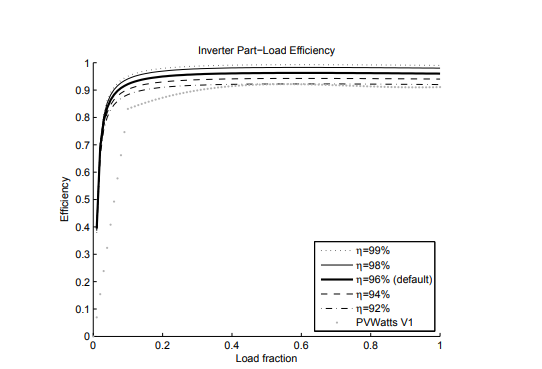
\includegraphics[width=0.8\textwidth]{images/inverter effiency.png}
    \caption{Inverter Part-Load Efficiency. This graph illustrates how inverter efficiency varies with the load fraction, showing different nominal efficiencies and a comparison to PVWatts V1.}
    \label{fig:inverter_efficiency}
\end{figure}
 
 \item \textbf{The Trade-off:} Assuming a constant efficiency (a simple linear model) is fast but leads to modeling inaccuracies and suboptimal economic results. $\text{PWL}$ modeling offers a better balance between \textbf{accuracy} and \textbf{computational complexity}.\end{itemize}\subsubsection*{2. Implementation Steps}The \textbf{Piecewise Linear Approximation ($\text{PWL}$)} transforms the curve into a set of linear functions, typically using the \textbf{Multiple Choice/Convex Combination approach} (also known as the $\lambda$-method or Special Ordered Sets of Type 2, $\text{SOS}2$):\begin{enumerate}\item \textbf{Define Segments/Breakpoints:} The non-linear curve is divided into $N$ linear segments defined by $N+1$ known points (breakpoints) along the input power axis. The accuracy increases with the number of segments, but so does the computational time.\item \textbf{Introduce Binary Variables (for segments):} You assign auxiliary $\text{binary variables}$ ($\delta_s$) to identify which segment is active at any given time step.\item \textbf{Use Convex Combination ($\lambda$-method):} The actual power flow point on the curve is represented as a convex combination of the segment breakpoints. This uses additional continuous variables ($\lambda_i$) whose sum must equal 1.
 \begin{itemize}
 \item $P_{dc} = \sum_{i} \lambda_i P_{dc, i}$ (The actual power is a weighted average of the breakpoint powers).
 \item $\eta(P_{dc}) = \sum_{i} \lambda_i \eta_i$ (The calculated efficiency is a weighted average of the breakpoint efficiencies).
 \end{itemize}
 Constraints ensure that only two adjacent $\lambda$ values (or their corresponding segment binary variables) can be non-zero simultaneously, forcing the solution to lie on a defined segment.
 \end{enumerate}

\subsection{Part-Load Operation HTHP}
\label{sub:part_load_modeling}
\subsubsection{Inverter modulated model}
The performance of a heat pump at a given temperature depends on its operating regime, which in turn alters the effective coefficient of performance. The effective COP, denoted as \textbf{$\mathrm{COP}^{\star}(\Delta T)$}, is defined by \ref{eq:cop_star_delta_t_new} based on different operating conditions \cite{Rogeau2024HPPL}:

\begin{equation}
\label{eq:cop_star_delta_t_new}
\mathrm{COP}^{\star}(\Delta T) =
\begin{cases}
\mathrm{COP}^{\mathrm{FL}}(\Delta T_{\mathrm{HP}}), & \text{if } T_{\mathrm{out}} \le T_{\mathrm{biv}} \\
\mathrm{COP}^{\mathrm{PL}}(\Delta T_{\mathrm{HP}}), & \text{if } T_{\mathrm{biv}} \le T_{\mathrm{out}} \le T_{\mathrm{biv}, 2} \\
\mathrm{COP}^{0/1}(\Delta T), & \text{if } T_{\mathrm{out}} \ge T_{\mathrm{biv}, 2}
\end{cases}
\end{equation}

The core operational principle of modern high-temperature heat pumps (HTHPs), such as the Daikin EWYE-CZ, relies on inverter technology (Variable Frequency Drive or VFD) to modulate power and maintain efficiency at partial load conditions. While this modulating behavior leads to higher realistic performance ($\mathrm{COP}^{\mathrm{PL}}$) by minimizing efficiency losses associated with frequent on/off cycling, its full integration into a design-and-operation Mixed-Integer Linear Program (MILP) introduces a significant modeling challenge. Precisely modeling regimes such as $\mathrm{COP}^{\star}(\Delta T)$ which transition from full load ($\mathrm{COP}^{\mathrm{FL}}$) to inverter-controlled ($\mathrm{COP}^{\mathrm{PL}}$) and eventually to on/off cycles ($\mathrm{COP}^{0/1}$) requires defining the non-linear performance curve using Piecewise Linear (PWL) approximations or introducing a matrix of auxiliary binary decision variables to select the active operating segment at every time step of the simulation. This drastic increase in discrete variables would expand the combinatorial search space of the MILP exponentially, making the computational problem intractable and violating the requirement for a functional, fast optimization tool. Therefore, for the sake of model simplicity and computational feasibility, the HP operation for all regimes, including the inverter-modulated segment, is conservatively simplified to a single on/off (full-load) switching mechanism, acknowledging that this design choice inherently leads to an underestimation of the HP's true seasonal performance (SCOP).
\subsubsection{Simplified model}
The estimation of Part Load (PL) performance for the heat pump assumes adherence to the EN 14511: 2022 standard, as detailed in relevant literature \cite{Grassi2018HP}.
\begin{equation}\label{eq:pl}\mathrm{COP}{\mathrm{PL}}[-] = (1 - C{\text{d}}(1 - \text{PLR}))\mathrm{COP} \quad \text{with} \quad \mathrm{PLR}[-] = \frac{\min(\dot{Q}{\text{demand}}, \dot{Q}{\text{duty}})}{\dot{Q}_{\text{duty}}}\end{equation}In \cref{eq:pl} , $C_{\text{d}} (-)$ represents the degradation coefficient, assigned a value of $0.25$ for air-to-water HP systems \cite{Grassi2018HP}.The $\text{PLR} (-)$ variable quantifies the part load ratio by comparing the required heating output against the maximum possible theoretical output under prevailing weather conditions.This maximum output is termed the duty $\dot{Q}_{\text{duty}} (\text{W})$, while the load actually required by the building is the heat demand $\dot{Q}_{\text{demand}} (\text{Wh/h or W})$, which may also be the effective heat to be provided.The duty is derived from the Lorenz $\text{COP}$ and the nominal power use, as defined by the sizing and setpoint temperature in \cref{eq: duty}.\begin{equation}\label{eq: duty}\dot{Q}{\text{duty}}[\mathrm{W}] = \mathrm{COP}{\mathrm{Lorenz}}\frac{\dot{Q}{\mathrm{HP,nom}}}{\mathrm{COP}{\mathrm{nom}}}\end{equation}In \cref{eq: duty}, $\dot{Q}_{\text{HP,nom}} (\text{W})$ is the sizing parameter used for HPs and $\text{COP}_{\text{nom}} (-)$ represents the nominal $\text{COP}$ linked to the system's target setpoint temperature. Finally, the electrical power drawn by the HP and the net heat provided to the load are calculated using the duty cycle, as shown in \ref{eq: duty_final}.
\begin{equation}
\label{eq: duty_final}
P_{\mathrm{HP}}[\mathrm{W}] = \min\left(\frac{\dot{Q}{\mathrm{demand}}}{\mathrm{COP}{\mathrm{PL}}}, \frac{\dot{Q}{\mathrm{duty}}}{\mathrm{COP}{\mathrm{PL}}}\right) \quad \text{and} \quad \dot{Q}{\mathrm{HP}}[\mathrm{W}] = \mathrm{COP}{\mathrm{PL}}P_{\mathrm{HP}}
\end{equation}

\section{Conclusion}
The literature reviewed in this chapter establishes a robust methodological foundation for the design and operation of complex, hybrid energy systems.
As the building sector shifts toward decarbonization, it is evident that static, rule-of-thumb dimensioning standards (such as EN 15450) are insufficient for systems integrating High-Temperature Heat Pumps (HTHPs), Photovoltaics (PV), Battery Energy Storage Systems (BESS), and Thermal Energy Storage (TES).
Achieving both economic viability and grid stability requires the simultaneous optimization of component sizing and operational scheduling.

Several key takeaways emerge from the evaluation of energy system modeling methodologies:

\begin{itemize}
    \item \textbf{The Suitability of MILP:} Mixed-Integer Linear Programming (MILP) stands out as the most appropriate mathematical framework for this application.
    Unlike heuristic methods (e.g., Genetic Algorithms or Particle Swarm Optimization) that only offer near-optimal approximations, MILP guarantees a deterministic, globally optimal solution.
    It natively handles the combination of continuous variables (e.g., energy flows, state of charge) and discrete binary decisions (e.g., investment choices, on/off operational states) required for co-optimizing system design and dispatch.
    
    \item \textbf{Balancing Accuracy and Tractability:} The primary limitation of MILP is its strict requirement for linear constraints.
    However, the literature demonstrates that complex, non-linear thermodynamic behaviors can be successfully integrated without causing computational bottlenecks.
    Techniques such as Piecewise Linear (PWL) approximations for inverter efficiencies, stratified 2-zone models for TES, and Lorentz-based or simplified part-load COP models for HTHPs provide the necessary balance between physical realism and solver efficiency.
    
    \item \textbf{Evaluating Trade-offs:} Multi-objective optimization, specifically utilizing the $\epsilon$-constraint method, provides a vital mechanism for evaluating competing goals.
    It allows for the clear visualization of trade-offs between minimizing the Total Cost of Ownership (TCO) and reducing life-cycle CO$_2$ emissions via Pareto fronts.
\end{itemize}

Ultimately, these modeling strategies validate the approach taken in this thesis.
By utilizing a MILP-based framework with carefully selected component linearizations, the proposed design tool is well-equipped to navigate the complex interdependencies of hybrid energy systems.
This methodology will directly enable the cost-optimal and environmentally sound transition from gas boilers to electrified heating for commercial applications like the M-accent case study.





%----------------------------------------------------------------------------------
%----------------------------------------------------------------------------------
%----------------------------------------------------------------------------------
%----------------------------------------------------------------------------------
%----------------------------------------------------------------------------------
%----------------------------------------------------------------------------------
%----------------------------------------------------------------------------------
%----------------------------------------------------------------------------------
%----------------------------------------------------------------------------------
%----------------------------------------------------------------------------------
%----------------------------------------------------------------------------------
%----------------------------------------------------------------------------------
%----------------------------------------------------------------------------------
%----------------------------------------------------------------------------------

%---------------------------------------------------------------------------------
%----------------------------------------------------------------------------------
%----------------------------------------------------------------------------------
%----------------------------------------------------------------------------------
%----------------------------------------------------------------------------------
%----------------------------------------------------------------------------------
%----------------------------------------------------------------------------------
%----------------------------------------------------------------------------------
%----------------------------------------------------------------------------------

\chapter{Methodology}
\label{chapt3}

The preceding chapters established the problem context and the theoretical foundation for this work.
Chapter~\ref{intro} identified the core challenge: replacing the two 80\,kW gas boilers at the M-accent commercial building with an electrified hybrid system comprising a High-Temperature Heat Pump (HTHP), Photovoltaic (PV) array, Battery Energy Storage System (BESS), and Thermal Energy Storage (TES) --- while simultaneously minimising the Total Cost of Ownership (TCO).
Chapter~\ref{literature review} reviewed the available optimisation paradigms and concluded that Mixed-Integer Linear Programming (MILP) is the most appropriate framework for this application: it guarantees a globally optimal solution, natively handles the mixed continuous-and-discrete decision structure inherent to energy systems, and integrates seamlessly with the time-varying electricity tariffs that drive economic dispatch decisions.

Building on those foundations, this chapter presents the complete mathematical formulation of the MILP design tool developed in this thesis.
The model co-optimises two interrelated decision layers: the \textit{investment layer}, which determines the optimal installed capacities of the HTHP, PV array, BESS, and TES; and the \textit{operational layer}, which determines the cost-optimal hourly dispatch of every technology over a representative full calendar year (8\,760 time steps).
These two layers cannot be solved independently: the economic value of storage, for instance, depends on how it is operated, and the optimal operating strategy in turn depends on the installed capacity.
The MILP formulation resolves this coupling in a single unified optimisation problem.

The chapter is structured as follows.
Section~\ref{sec:data_inputs} describes the input data pipeline: the climatic, tariff, and load profiles that drive the model.
Sections~\ref{sec:hthp_model}--\ref{sec:tes_model} develop the linearised component models for each technology, detailing the physical constraints and the linearisation choices required for MILP compatibility.
Section~\ref{sec:energy_balance} states the system-level energy balance constraints that couple all components at every time step.
Section~\ref{sec:objective_function} defines the objective function, which minimises the annualised total system cost comprising CAPEX and OPEX.
Finally, Section~\ref{sec:solver_settings} documents the solver configuration and solution strategy.

% ============================================================
\section{Input Data and Pre-Processing}
\label{sec:data_inputs}
% ============================================================

% TODO: Describe the five hourly time-series datasets (8760 time steps):
%   - Day-ahead electricity spot prices  lambda(t)  [EUR/kWh]
%   - Solar irradiance G(t) [W/m^2] and ambient temperature T_amb(t)  from TMY file
%   - Thermal heat demand Q_dem(t) [kW] of the M-accent building
%   - Electrical demand P_dem(t) [kW] of the M-accent building
%   - Grid connection constraints: max import/export power P_max, network tariffs
%
% TODO: Explain data sources (Elia EPEX spot prices, EnergyPlus TMY, building metering data)
% TODO: Describe normalisation, validation, and alignment to common hourly resolution
% TODO: Describe identification of representative operational periods (seasonal, peak, off-peak)

% ============================================================
\section{Techno-Economic Parameters}
\label{sec:econ_params}
% ============================================================

Before presenting the component models it is necessary to establish the economic framework
used to translate one-time capital expenditures into annual costs comparable with the
annual operational expenditures optimised by the MILP.
This section describes the Capital Recovery Factor, the economies-of-scale cost model,
and lists all techno-economic parameters used in the study.

% ------------------------------------------------------------
\subsection{Capital Recovery Factor (CRF)}
\label{sub:crf}
% ------------------------------------------------------------

Investment costs for all technologies are converted to an equivalent \textbf{annualised
CAPEX} using the Capital Recovery Factor (CRF), also known as the annuity factor.
The CRF spreads a one-time investment over the asset's economic lifetime $n$ [yr]
at a fixed discount rate $r$ [-], representing the weighted average cost of capital (WACC):

\begin{equation}
    \mathrm{CRF}(r,\,n) = \frac{r\,(1+r)^{n}}{(1+r)^{n}-1}.
    \label{eq:crf}
\end{equation}

\noindent A single discount rate of $r = 5\,\%$ is applied uniformly to all technologies,
reflecting a typical WACC for commercial building energy investments in Belgium~\cite{VEKA2026}.
Each technology has its own economic lifetime $n$, so a separate CRF value is computed per
technology.
The annualised CAPEX for a technology with unit investment cost $c$ [\euro/unit] and
installed capacity $X$ [unit] is then:

\begin{equation}
    \mathrm{CAPEX}_\mathrm{ann}(X) = c \cdot \mathrm{CRF}(r,n) \cdot X
    \quad [\text{\euro/yr}].
    \label{eq:capex_ann_linear}
\end{equation}

\noindent In reality, the specific cost $c$ depends on the scale of installation, which
is addressed by the economies-of-scale model described next.

% ------------------------------------------------------------
\subsection{Economies-of-Scale Cost Model}
\label{sub:eos}
% ------------------------------------------------------------

Large installations benefit from lower specific (per-unit) costs due to procurement
discounts, fixed installation overheads spread over greater capacity, and engineering
efficiency.
This is captured by a \textbf{power-law} (``six-tenths rule'') scaling of total annual
cost with installed capacity~\cite{Shafer2006EOS}:

\begin{equation}
    \mathrm{CAPEX}_\mathrm{ann}(X)
    = c_\mathrm{ref} \cdot X_\mathrm{ref}
      \left(\frac{X}{X_\mathrm{ref}}\right)^{\!\alpha},
    \quad \alpha = 0.6,
    \label{eq:eos}
\end{equation}

\noindent where $X_\mathrm{ref}$ is the reference (anchor) capacity at which the
specific cost $c_\mathrm{ref}$ [\euro/unit/yr] is exactly known from market data,
and $\alpha = 0.6$ is the industry-standard scaling exponent.
Because $\alpha < 1$ the function is concave: the marginal cost decreases as capacity
grows.

The power-law curve is inherently non-linear and cannot be embedded directly in the MILP.
It is therefore approximated by a \textbf{piecewise-linear} (PWL) function using Gurobi's
native \texttt{addGenConstrPWL} constraint, with breakpoints distributed using quadratic
spacing to cluster more points near zero capacity where the curvature is steepest.
This approximation preserves the concavity of the cost curve and therefore does not affect
the global optimality guarantee of the solver.

% ------------------------------------------------------------
\subsection{Technology Parameters}
\label{sub:tech_params}
% ------------------------------------------------------------

\autoref{tab:econ_params} lists all techno-economic parameters used in the MILP model.
The unit CAPEX values are based on current Belgian market data and recent literature for
each technology.

\begin{table}[H]
\centering
\caption{Techno-economic parameters for all candidate technologies.
         CRF values computed with $r = 5\,\%$ via \eqref{eq:crf}.
         Annualised CAPEX is the product of unit CAPEX and CRF, evaluated at the
         EOS anchor capacity.}
\label{tab:econ_params}
\begin{tabular}{lcccccc}
\hline
\textbf{Technology} & \textbf{Unit} & \textbf{CAPEX} & \textbf{Lifetime} & \textbf{CRF} & \textbf{Ann.\ CAPEX} & \textbf{EOS anchor} \\
                    &               & [\text{\euro}/unit]   & [yr]              & [-]          & [\text{\euro}/unit/yr]      & [unit] \\
\hline
HTHP (Daikin EWYE-CZ) & kW$_\mathrm{th}$ & 7\,000 & 20 & 0.0802 & 561.7 & 30\,kW$_\mathrm{th}$ \\
PV array              & kW$_\mathrm{p}$  &   900  & 25 & 0.0710 &  63.9 & 10\,kW$_\mathrm{p}$ \\
BESS                  & kWh              &   800  & 15 & 0.0963 &  77.1 & 10\,kWh \\
LTES (PCM)            & kWh$_\mathrm{th}$ & 600   & 20 & 0.0802 &  48.1 & 30\,kWh$_\mathrm{th}$ \\
WTES (water tank)     & kWh$_\mathrm{th}$ & 132.5 & 20 & 0.0802 &  10.6 & 3.3\,kWh$_\mathrm{th}$ \\
\hline
\end{tabular}
\end{table}

\noindent The WTES reference cost is derived from a market benchmark of
$3\,\text{\euro}/\text{L}$ at a 500\,L tank~\cite{Krien2020oemofsolph}, converted to a
specific energy cost using the water thermal capacity
($\rho c_p = 971.8 \times 4190\,\mathrm{J/(m^3\cdot K)}$) over a temperature
swing of $\Delta T = 20\,\mathrm{K}$ (supply $60\,^{\circ}$C,
return $40\,^{\circ}$C), yielding $22.6\,\mathrm{kWh_{th}/m^3}$ and a
unit cost of $132.5\,\text{\euro}/\mathrm{kWh_{th}}$.

% ------------------------------------------------------------
\subsection{Other Economic Parameters}
\label{sub:other_econ}
% ------------------------------------------------------------

\autoref{tab:other_econ} lists the remaining economic parameters that appear in the
objective function but are not technology-specific investment costs.

\begin{table}[H]
\centering
\caption{Other economic parameters used in the objective function.}
\label{tab:other_econ}
\begin{tabular}{lcc}
\hline
\textbf{Parameter} & \textbf{Value} & \textbf{Unit} \\
\hline
Discount rate (WACC)            & 5.0   & \% \\
VAT on operational costs        & 21.0  & \% \\
Capacity network tariff         & 5.0   & \euro/kW/month \\
Fixed annual connection cost    & 200   & \euro/yr \\
Maximum annual CAPEX budget     & 250\,000 & \euro/yr \\
EOS scaling exponent $\alpha$   & 0.6   & --- \\
\hline
\end{tabular}
\end{table}

\noindent The capacity tariff of $5\,\text{\euro/kW/month}$ reflects the Belgian
distribution network tariff structure, where the monthly peak grid import power
determines a significant fraction of the network cost.
This tariff creates a strong incentive for the MILP to smooth and reduce peak grid
imports, which in turn motivates investment in the BESS and TES.

% ============================================================
\section{Component Models}
\label{sec:component_models}
% ============================================================

This section presents the linearised mathematical models for each technology in the candidate system.
All models are formulated as linear equality and inequality constraints suitable for direct embedding in the MILP problem.

% ------------------------------------------------------------
\subsection{High-Temperature Heat Pump (HTHP)}
\label{sec:hthp_model}
% ------------------------------------------------------------

The High-Temperature Heat Pump (HTHP) is the primary source of thermal energy in the system,
converting electrical power into heat at supply temperatures up to $75\,^{\circ}\mathrm{C}$,
making it suitable for the existing radiator circuit of the M-accent building without requiring
hydronic renovation.
The specific unit modelled is the Daikin EWYE-CZ air-to-water heat pump; its full manufacturer
datasheet is reproduced in Appendix~\ref{appendix:datasheet_hthp}.

Two ambient-temperature-dependent effects must be captured simultaneously: the change in
thermodynamic \emph{efficiency} (COP) and the change in physically \emph{available capacity}
(rated thermal output).
These are treated as two separate pre-computed parameter arrays, described next, which are then
embedded as fixed coefficients in the MILP constraints.

% - - - - - - - - - - - - - - - - - - - - - - - - - - - - - - -
\subsubsection{Pre-Processing Step 1: Lorentz COP Time Series}
\label{sub:hthp_cop_preprocess}
% - - - - - - - - - - - - - - - - - - - - - - - - - - - - - - -

As established in Section~\ref{sub:lorentz_model}, the Lorentz model expresses the ideal COP
of a heat pump in terms of the log-mean temperatures on the condenser (sink) side and the
evaporator (source) side.
With a fixed supply temperature $T_\mathrm{sup}$ [$^{\circ}$C] and fixed return temperature
$T_\mathrm{ret}$ [$^{\circ}$C], the log-mean condenser temperature is a constant:

\begin{equation}
    T_{\mathrm{h,lm}} =
    \frac{T_\mathrm{sup} - T_\mathrm{ret}}
         {\ln\!\left(\dfrac{T_\mathrm{sup}+273.15}{T_\mathrm{ret}+273.15}\right)}
    \quad [\mathrm{K}].
    \label{eq:T_hlm}
\end{equation}

The heat source is outdoor air at the hourly ambient temperature $T_\mathrm{amb}(t)$
[$^{\circ}$C], converted to Kelvin as $T_\mathrm{src}(t) = T_\mathrm{amb}(t)+273.15$~[K].
The ideal Lorentz COP at each hour is therefore:

\begin{equation}
    \mathrm{COP}_\mathrm{Lorenz}(t)
    = \frac{T_{\mathrm{h,lm}}}{T_{\mathrm{h,lm}} - T_\mathrm{src}(t)}.
    \label{eq:cop_lorenz_t}
\end{equation}

The actual COP is obtained by scaling with the Lorentz efficiency factor
$\eta_\mathrm{HP}$, calibrated from manufacturer performance data
(Appendix~\ref{appendix:datasheet_hthp}) at the reference operating point:

\begin{equation}
    \mathrm{COP}(t) = \eta_\mathrm{HP} \cdot \mathrm{COP}_\mathrm{Lorenz}(t),
    \qquad \eta_\mathrm{HP} = 0.361.
    \label{eq:cop_actual_t}
\end{equation}

\noindent Because both $T_\mathrm{h,lm}$ and $\eta_\mathrm{HP}$ are constants, and
$T_\mathrm{amb}(t)$ is a known input time series, $\mathrm{COP}(t)$ is fully determined
before the optimisation begins.
It is passed to Gurobi as a \emph{scalar parameter} at each time step, making every
constraint in which it appears linear.

% - - - - - - - - - - - - - - - - - - - - - - - - - - - - - - -
\subsubsection{Pre-Processing Step 2: Capacity-Fraction Linear Regression}
\label{sub:hthp_capfrac}
% - - - - - - - - - - - - - - - - - - - - - - - - - - - - - - -

At low ambient temperatures an air-source heat pump cannot deliver its rated thermal output:
the refrigerant mass-flow rate decreases as the evaporator pressure drops.
This effect is \emph{separate} from the COP variation and must be modelled independently as
a reduction in the \emph{available} capacity.

A \textbf{linear regression} is fitted to the heating-capacity data extracted from the
Daikin EWYE-CZ manufacturer simulation at full load and a fixed condenser leaving water
temperature of $55\,^{\circ}$C (eight points from $-15\,^{\circ}$C to $+7\,^{\circ}$C
plus one high-temperature point at $+20\,^{\circ}$C).
The regression is forced through the reference point $(T_\mathrm{ref} = 7\,^{\circ}\mathrm{C},\;
\kappa = 1.0)$, yielding:

\begin{equation}
    \kappa(t) = 1 + k \bigl(T_\mathrm{amb}(t) - T_\mathrm{ref}\bigr),
    \quad k = 0.02106\,^{\circ}\mathrm{C}^{-1},\quad T_\mathrm{ref} = 7\,^{\circ}\mathrm{C},
    \label{eq:capfrac}
\end{equation}

\noindent clipped to the manufacturer operating envelope:
$\kappa(t) \in [0.537,\; 1.274]$ (corresponding to
$T_\mathrm{amb} \in [-15\,^{\circ}\mathrm{C},\; +20\,^{\circ}\mathrm{C}]$).
The fit achieves $R^2 = 0.997$.
Like $\mathrm{COP}(t)$, the array $\kappa(t)$ is pre-computed and enters the MILP
as a fixed coefficient.

\noindent \textbf{Physical interpretation.}
A value $\kappa < 1$ means the unit can deliver less than its nameplate output at cold
conditions; a value $\kappa > 1$ means it can slightly exceed nameplate at mild conditions.
The effective weather-derated capacity at any hour is therefore
$Q_\mathrm{hp}^{*} \cdot \kappa(t)$ [kW].

% - - - - - - - - - - - - - - - - - - - - - - - - - - - - - - -
\subsubsection{MILP Decision Variables}
% - - - - - - - - - - - - - - - - - - - - - - - - - - - - - - -

The MILP introduces the following variables for the HTHP:

\begin{itemize}
    \item $Q_\mathrm{hp}^{*} \in [0,\; Q_\mathrm{hp,max}^{*}]$ [kW$_\mathrm{th}$] ---
          continuous sizing variable (rated thermal output at reference conditions).
    \item $u_\mathrm{HP}(t) \in \{0,1\}$ --- binary on/off commitment at time step $t$.
    \item $\tilde{Q}_\mathrm{hp}(t) \geq 0$ [kW$_\mathrm{th}$] --- auxiliary continuous
          variable equal to $Q_\mathrm{hp}^{*}$ when $u_\mathrm{HP}(t)=1$ and zero
          otherwise (linearises the product $Q_\mathrm{hp}^{*} \cdot u_\mathrm{HP}(t)$).
    \item $Q_\mathrm{HP}(t) \geq 0$ [kW$_\mathrm{th}$] --- actual thermal output delivered.
    \item $P_\mathrm{el,HP}(t) \geq 0$ [kW$_\mathrm{el}$] --- electrical power consumed.
\end{itemize}

% - - - - - - - - - - - - - - - - - - - - - - - - - - - - - - -
\subsubsection{On/Off Linearisation (Big-$M$)}
% - - - - - - - - - - - - - - - - - - - - - - - - - - - - - - -

The auxiliary variable $\tilde{Q}_\mathrm{hp}(t)$ linearises the bilinear product
$Q_\mathrm{hp}^{*} \cdot u_\mathrm{HP}(t)$ via the standard three-constraint big-$M$
formulation:

\begin{align}
    \tilde{Q}_\mathrm{hp}(t) &\leq Q_\mathrm{hp,max}^{*}\, u_\mathrm{HP}(t)
        \label{eq:hthp_bigm1} \\
    \tilde{Q}_\mathrm{hp}(t) &\leq Q_\mathrm{hp}^{*}
        \label{eq:hthp_bigm2} \\
    \tilde{Q}_\mathrm{hp}(t) &\geq Q_\mathrm{hp}^{*} - Q_\mathrm{hp,max}^{*}\,
        \bigl(1 - u_\mathrm{HP}(t)\bigr).
        \label{eq:hthp_bigm3}
\end{align}

\noindent When $u_\mathrm{HP}(t)=0$, constraints \eqref{eq:hthp_bigm1} and
\eqref{eq:hthp_bigm3} together force $\tilde{Q}_\mathrm{hp}(t)=0$.
When $u_\mathrm{HP}(t)=1$, constraints \eqref{eq:hthp_bigm2} and \eqref{eq:hthp_bigm3}
together force $\tilde{Q}_\mathrm{hp}(t)=Q_\mathrm{hp}^{*}$.

% - - - - - - - - - - - - - - - - - - - - - - - - - - - - - - -
\subsubsection{Thermal Output Bounds}
% - - - - - - - - - - - - - - - - - - - - - - - - - - - - - - -

The actual thermal output is bounded by the weather-derated capacity from above and by a
minimum load fraction $f_\mathrm{min}$ from below (set to $0.222$ from manufacturer data):

\begin{align}
    Q_\mathrm{HP}(t) &\leq \tilde{Q}_\mathrm{hp}(t)\cdot\kappa(t)
        \label{eq:hthp_qmax} \\
    Q_\mathrm{HP}(t) &\geq f_\mathrm{min}\,\tilde{Q}_\mathrm{hp}(t)\cdot\kappa(t).
        \label{eq:hthp_qmin}
\end{align}

\noindent Since $\kappa(t)$ is a pre-computed scalar, both constraints remain linear in
the decision variables $Q_\mathrm{HP}(t)$ and $\tilde{Q}_\mathrm{hp}(t)$.
The lower bound prevents unrealistically shallow cycling; the electric boiler covers any
residual demand that the HTHP cannot meet at minimum load.

% - - - - - - - - - - - - - - - - - - - - - - - - - - - - - - -
\subsubsection{Electrical Power with On/Off Cycling Penalty}
\label{sub:hthp_power}
% - - - - - - - - - - - - - - - - - - - - - - - - - - - - - - -

A purely ideal model would set $P_\mathrm{el,HP}(t) = Q_\mathrm{HP}(t)/\mathrm{COP}(t)$.
However, on/off cycling incurs compressor restart losses that cause the unit to consume
some electrical power even below its minimum thermal output.
Following the EN~14511 part-load degradation approach reviewed in
Section~\ref{sub:part_load_modeling}, this is captured by a degradation coefficient
$C_\mathrm{d}$ that splits the electrical draw into a fixed fraction proportional to the
\emph{derated rated capacity} and a variable fraction proportional to the \emph{actual output}:

\begin{equation}
    P_\mathrm{el,HP}(t)\cdot\mathrm{COP}(t)
    = C_\mathrm{d}\,\tilde{Q}_\mathrm{hp}(t)\cdot\kappa(t)
      + \bigl(1-C_\mathrm{d}\bigr)\,Q_\mathrm{HP}(t),
    \quad C_\mathrm{d} = 0.10.
    \label{eq:hthp_power}
\end{equation}

\noindent Because $\mathrm{COP}(t)$ and $\kappa(t)$ are fixed parameters, the right-hand
side is linear in $\tilde{Q}_\mathrm{hp}(t)$ and $Q_\mathrm{HP}(t)$, and the
left-hand side is linear in $P_\mathrm{el,HP}(t)$.
The constraint is therefore directly embeddable in the MILP.

To verify consistency: at full load ($Q_\mathrm{HP} = \tilde{Q}_\mathrm{hp}\cdot\kappa$)
equation~\eqref{eq:hthp_power} reduces to
$P_\mathrm{el,HP}\cdot\mathrm{COP} = \tilde{Q}_\mathrm{hp}\cdot\kappa = Q_\mathrm{HP}$,
i.e.\ $P_\mathrm{el,HP} = Q_\mathrm{HP}/\mathrm{COP}$, recovering the ideal relation.
At output below rated, the $C_\mathrm{d}$ term adds a fixed overhead that reduces the
effective part-load COP, consistent with the cycling-loss mechanism described in
Section~\ref{sub:part_load_modeling}.

% - - - - - - - - - - - - - - - - - - - - - - - - - - - - - - -
\subsubsection{Summary of HTHP Constraints}
% - - - - - - - - - - - - - - - - - - - - - - - - - - - - - - -

Table~\ref{tab:hthp_constraints} collects all HTHP constraints, the pre-computed
parameters they use, and their role in the MILP.

\begin{table}[H]
\centering
\caption{Complete HTHP constraint set embedded in the MILP.
         $\kappa(t)$ and $\mathrm{COP}(t)$ are pre-computed parameter arrays;
         all other symbols are MILP variables.}
\label{tab:hthp_constraints}
\begin{tabular}{llp{5.5cm}}
\hline
\textbf{Label} & \textbf{Constraint} & \textbf{Role} \\
\hline
\eqref{eq:hthp_bigm1}--\eqref{eq:hthp_bigm3}
    & Big-$M$ on $\tilde{Q}_\mathrm{hp}(t)$
    & Links sizing variable to on/off binary \\
\eqref{eq:hthp_qmax}
    & $Q_\mathrm{HP}(t) \leq \tilde{Q}_\mathrm{hp}(t)\,\kappa(t)$
    & Weather-derated upper capacity \\
\eqref{eq:hthp_qmin}
    & $Q_\mathrm{HP}(t) \geq f_\mathrm{min}\,\tilde{Q}_\mathrm{hp}(t)\,\kappa(t)$
    & Minimum load fraction \\
\eqref{eq:hthp_power}
    & $P_\mathrm{el}\,\mathrm{COP}(t) = C_\mathrm{d}\tilde{Q}\kappa + (1-C_\mathrm{d})Q_\mathrm{HP}$
    & Electrical draw with cycling penalty \\
\hline
\end{tabular}
\end{table}

% ------------------------------------------------------------
\subsection{Photovoltaic (PV) Array}
\label{sec:pv_model}
% ------------------------------------------------------------

The PV array provides on-site renewable electricity, directly offsetting grid imports and
supplying the HTHP, BESS, and building loads.
Its MILP representation is intentionally simple: all complex photovoltaic physics
(plane-of-array irradiance, cell temperature derating, DC-to-AC inverter losses,
soiling, and wiring losses) are handled entirely in a pre-processing step using the
PVGIS tool, so only a single linear constraint is needed inside the optimiser.

% - - - - - - - - - - - - - - - - - - - - - - - - - - - - - -
\subsubsection{Pre-Processing: Normalised AC Output from PVGIS}
% - - - - - - - - - - - - - - - - - - - - - - - - - - - - - -

The European Commission's PVGIS API~\cite{Huld2012PVGIS} is used to generate an
hourly AC power time series for the M-accent building location
(Brussels, $50.85^{\circ}$N, $4.35^{\circ}$E) for the reference year 2023.
The query is submitted for a normalised 1\,kW$_\mathrm{p}$ system with a fixed tilt
of $35^{\circ}$ and a total system loss of 14\,\% (covering wiring, shading, soiling,
and temperature derating).
PVGIS internally computes the full PV yield chain --- irradiance transposition to the
tilted plane, cell temperature correction, and DC-to-AC conversion --- and returns the
result as a single hourly array:

\begin{equation}
    I_\mathrm{sol}(t) \quad [\mathrm{kW/kW_p}], \qquad t = 1, \ldots, 8760.
    \label{eq:pvgis_output}
\end{equation}

\noindent This normalised specific yield is stored as a fixed parameter array before
the optimisation begins.
Delegating the PV physics to PVGIS avoids introducing any non-linear terms
(e.g.\ the cell temperature correction $1 + \gamma_\mathrm{pdc}(T_\mathrm{cell}-T_\mathrm{ref})$)
into the MILP, while still capturing realistic seasonal and diurnal generation profiles.

% - - - - - - - - - - - - - - - - - - - - - - - - - - - - - -
\subsubsection{Decision Variable and Technology-Selection Binary}
% - - - - - - - - - - - - - - - - - - - - - - - - - - - - - -

The investment decision is the \textbf{installed peak capacity}:
\begin{equation}
    C_\mathrm{PV} \in [0,\; C_\mathrm{PV,max}] \quad [\mathrm{kW_p}],
    \label{eq:pv_sizing}
\end{equation}
with $C_\mathrm{PV,max} = 50\,\mathrm{kW_p}$ reflecting the available roof area of the
M-accent building.

A binary variable $y_\mathrm{PV} \in \{0,1\}$ indicates whether PV is installed at all.
This is required because the capital cost function is concave (economies of scale,
Section~\ref{sub:pv_capex}): without the binary, the optimizer could exploit the lower
per-unit cost at large capacity to install a negligibly small system at zero cost.
The technology-selection constraint is:
\begin{equation}
    C_\mathrm{PV} \leq C_\mathrm{PV,max}\, y_\mathrm{PV}.
    \label{eq:pv_select}
\end{equation}

% - - - - - - - - - - - - - - - - - - - - - - - - - - - - - -
\subsubsection{Hourly Generation Constraint}
% - - - - - - - - - - - - - - - - - - - - - - - - - - - - - -

The AC power injected by the PV array at each time step is simply:
\begin{equation}
    P_\mathrm{PV}(t) = I_\mathrm{sol}(t)\cdot C_\mathrm{PV},
    \qquad \forall\, t.
    \label{eq:pv_power}
\end{equation}

\noindent Since $I_\mathrm{sol}(t)$ is a known scalar parameter, this is linear in the
single decision variable $C_\mathrm{PV}$.
$P_\mathrm{PV}(t)$ enters the electrical energy balance
(Section~\ref{sec:energy_balance}) as a generation term.

% - - - - - - - - - - - - - - - - - - - - - - - - - - - - - -
\subsubsection{Grid-Injection Limit}
% - - - - - - - - - - - - - - - - - - - - - - - - - - - - - -

To prevent the model from selling grid-purchased electricity at a profit (a physically
impossible arbitrage), the power sold to the grid is capped at the sum of PV generation
and battery discharge:
\begin{equation}
    P_\mathrm{sell}(t) \leq P_\mathrm{PV}(t) + P_\mathrm{bat,dis}(t),
    \qquad \forall\, t.
    \label{eq:pv_sellcap}
\end{equation}

% - - - - - - - - - - - - - - - - - - - - - - - - - - - - - -
\subsubsection{Piecewise-Linear CAPEX with Economies of Scale}
\label{sub:pv_capex}
% - - - - - - - - - - - - - - - - - - - - - - - - - - - - - -

In practice, larger PV installations benefit from lower specific installation costs.
This is modelled with a \textbf{power-law cost curve}~\cite{Shafer2006EOS} using a
scaling exponent of $0.6$ (the industry-standard ``six-tenths rule''):

\begin{equation}
    \mathrm{CAPEX}_\mathrm{PV}(C_\mathrm{PV})
    = c_\mathrm{ref}\, C_\mathrm{ref}
      \left(\frac{C_\mathrm{PV}}{C_\mathrm{ref}}\right)^{0.6}
    \quad [\text{\euro/yr}],
    \label{eq:pv_capex_eos}
\end{equation}

\noindent where $c_\mathrm{ref} = 63.9\,\text{\euro/kW}_\mathrm{p}/\text{yr}$
(annualised from $900\,\text{\euro/kW}_\mathrm{p}$ over 25\,yr at 5\,\% discount rate)
and the anchor capacity is $C_\mathrm{ref} = 10\,\mathrm{kW_p}$.
Because equation~\eqref{eq:pv_capex_eos} is non-linear, it is approximated by a
\textbf{piecewise-linear} (PWL) function using Gurobi's native
\texttt{addGenConstrPWL} with breakpoints clustered near zero (quadratic spacing)
where the curve bends most steeply.
The PWL approximation preserves the concavity of the cost curve and therefore does
not affect the global optimality guarantee of the MILP solver.

% ------------------------------------------------------------
\subsection{Battery Energy Storage System (BESS)}
\label{sec:bess_model}
% ------------------------------------------------------------

% TODO: Sizing variables: energy capacity E* [kWh] and rated power P* [kW]
% TODO: State-of-charge (SOC) dynamics:  SOC(t+1) = SOC(t) + eta_ch*P_ch(t)*dt - P_dis(t)/eta_dis*dt
% TODO: SOC bounds: SOC_min * E* <= SOC(t) <= SOC_max * E*
% TODO: Charge/discharge power limits: 0 <= P_ch(t) <= P* * u_ch(t)
%                                      0 <= P_dis(t) <= P* * u_dis(t)
% TODO: Mutual exclusivity constraint: u_ch(t) + u_dis(t) <= 1
% TODO: Cyclic boundary condition: SOC(T) = SOC(1)

% ------------------------------------------------------------
\subsection{Thermal Energy Storage (TES)}
\label{sec:tes_model}
% ------------------------------------------------------------

% TODO: Sizing variable: tank volume V_tes* [m^3]  (linked to nominal capacity Q_N)
% TODO: Thermal energy balance: Q_TES(t+1) = Q_TES(t) + Q_ch,TES(t) - Q_dis,TES(t) - Q_loss(t)
% TODO: Heat loss model: Q_loss(t) = gamma * (T_in - T_amb(t)) * V_tes*  (linear in V_tes*)
% TODO: Capacity bounds: 0 <= Q_TES(t) <= Q_N(V_tes*)
% TODO: Charging/discharging power limits linked to HTHP rated output
% TODO: Cyclic boundary condition

% ------------------------------------------------------------
\subsection{Electric Boiler (Auxiliary Heater)}
\label{sec:eboiler_model}
% ------------------------------------------------------------

% TODO: Supplementary thermal source to cover peak demands or low-temperature HP lock-out periods
% TODO: Fixed or sized rated output Q_eb* [kW]
% TODO: Simple linear model: Q_eb(t) = eta_eb * P_eb(t),  binary on/off u_eb(t)
% TODO: Capacity constraint: Q_eb(t) <= Q_eb* * u_eb(t)

% ============================================================
\section{System Energy Balance Constraints}
\label{sec:energy_balance}
% ============================================================

% TODO: Electrical balance at every time step t:
%   P_PV(t) + P_dis(t) + P_grid,import(t)
%       = P_dem(t) + P_el,HP(t) + P_eb(t) + P_ch(t) + P_grid,export(t)
%
% TODO: Thermal balance at every time step t:
%   Q_HP(t) + Q_eb(t) + Q_dis,TES(t) = Q_dem(t) + Q_ch,TES(t)
%
% TODO: Grid import/export limits: 0 <= P_grid,import(t) <= P_max
%                                  0 <= P_grid,export(t) <= P_max
% TODO: Non-simultaneity of import and export (binary auxiliary variable or big-M)

% ============================================================
\section{Objective Function}
\label{sec:objective_function}
% ============================================================

% TODO: Minimise total annualised system cost:
%   min  CAPEX_annualised(x) + OPEX(u(t))
%
% TODO: CAPEX terms (annualised via Annuity Factor ANF):
%   - HTHP:  c_HTHP * Q_hp*  * ANF_HTHP
%   - PV:    c_PV   * A_pv*  * ANF_PV
%   - BESS:  c_BESS_E * E*  +  c_BESS_P * P*   (energy + power component)  * ANF_BESS
%   - TES:   c_TES  * V_tes* * ANF_TES
%   - E-boiler: c_eb * Q_eb*  * ANF_eb
%
% TODO: OPEX terms (summed over all 8760 time steps):
%   - Electricity purchase cost:  sum_t  lambda(t) * P_grid,import(t) * dt
%   - Feed-in revenue (if applicable): - sum_t  lambda_fit(t) * P_grid,export(t) * dt
%   - Capacity/network tariff on peak demand
%
% TODO: State Annuity Factor formula:  ANF = r*(1+r)^n / ((1+r)^n - 1)
%       with discount rate r and asset lifetime n

% ============================================================
\section{Solver Configuration and Solution Strategy}
\label{sec:solver_settings}
% ============================================================

% TODO: Solver: Gurobi (commercial) or CBC (open-source) via PuLP / Pyomo in Python
% TODO: Relative MIP optimality gap tolerance: 0.1 %
% TODO: Time limit: 3600 s
% TODO: Warm-start strategy (if used)
% TODO: Representative-period approach: describe any time-series clustering/reduction used
%       to keep the problem tractable (e.g. typical weeks, seasonal representative days)
% TODO: Hardware / computational environment used for results








%----------------------------------------------------------------------------------------------------------------------------------------------------------------------------------------------------------------------------------------
%-----------------------------------------------------------------------------
%-----------------------------------------------------------------------------
%-----------------------------------------------------------------------------
%-----------------------------------------------------------------------------
%-----------------------------------------------------------------------------
%-----------------------------------------------------------------------------
%-----------------------------------------------------------------------------
%-----------------------------------------------------------------------------
%-----------------------------------------------------------------------------
%-----------------------------------------------------------------------------
%-----------------------------------------------------------------------------
%-----------------------------------------------------------------------------
%-----------------------------------------------------------------------------
%-----------------------------------------------------------------------------
%-----------------------------------------------------------------------------
%-----------------------------------------------------------------------------

\bibliographystyle{unsrt}
\bibliography{bibliography.bib}
\addcontentsline{toc}{chapter}{Bibliography}

\appendix

\chapter{Datasheet HTHP Daikin EWYE-CZ}
\label{appendix:datasheet_hthp}


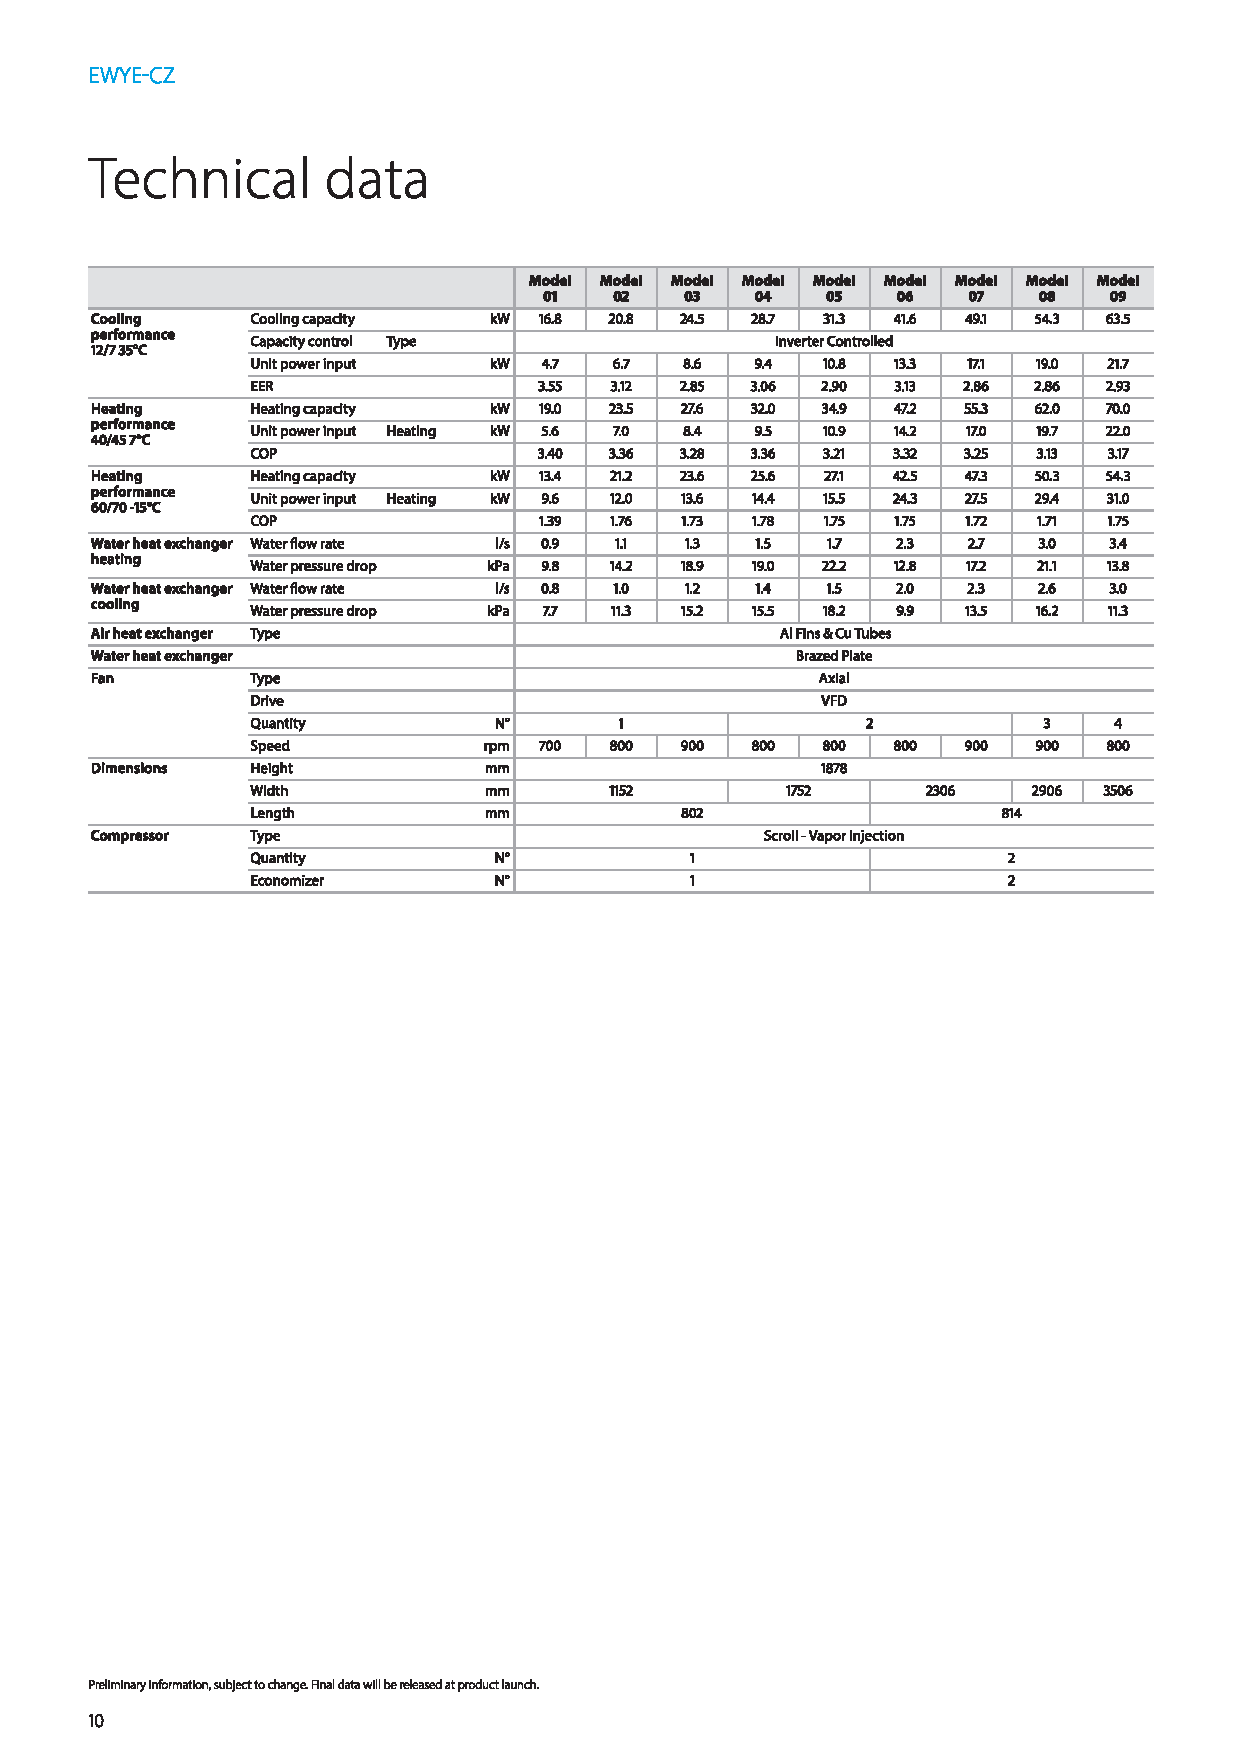
\includepdf{Appendices/DatasheetHTHP.pdf}






\includepdf[scale = 0.75, pages=1, pagecommand = \chapter{Title appendix B} \label{appendix:B}, offset=0cm -3cm]{Appendices/AppendixB.pdf}




\end{document}
